\documentclass{article}
\usepackage[utf8]{inputenc}
\usepackage{latexsym}
\usepackage{url}
\usepackage{hyperref}
\usepackage{graphicx}
\usepackage[table]{xcolor}
\usepackage[T1]{fontenc} 
\usepackage{LobsterTwo}
\usepackage{amsmath} %for math operations
\usepackage{fancyhdr} %for page style
\usepackage{lastpage} %for no of page
\usepackage[a4paper, total={6in, 8in}]{geometry} %for margins
\usepackage{geometry}
\geometry{right=24mm,left=24mm,top=45mm,bottom=45mm} %for page size 
\usepackage{bookman}
\usepackage{array}
\usepackage{wrapfig}
\usepackage{multirow}
\usepackage{tabularx}
\usepackage{amssymb}
\hypersetup{
     colorlinks=true, % make the links colored
     linkcolor=red,   % make the links colored
     urlcolor=blue    % make the URL colored
    }
\graphicspath{ {figures/} }
\color{black}
\setlength{\parindent}{4em}
\setlength{\parskip}{1em}
\renewcommand{\baselinestretch}{1}
\pagestyle{fancy}
\fancyhf{}
\rhead{\textcolor{blue}{\bfseries{$\copyright$}} Andreea Drăghici}
\renewcommand{\headrulewidth}{1pt}
\renewcommand{\footrulewidth}{1pt}
\rfoot{\textcolor{blue}{\textbf{Pagina}} \textbf \thepage \hspace{1pt} \textcolor{blue}{\textbf{din}} \pageref{LastPage}}
\renewcommand*\abstractname{\textcolor{red}{Rezumat}}
\renewcommand*\refname{\textcolor{red}{Referinte bibliografice}}
\renewcommand{\figurename}{Figura}
\renewcommand*\contentsname{
    \begin{abstract}
      Acest raport este o introducere in obiectivele de dezvoltare a temei de casa la disciplina Inteligenta Artificiala.
    \end{abstract}   
    \centering \textcolor{red}{ Introducere cuprins }}
\begin{document}
\slshape
\normalsize
\upshape
\sffamily
\begin{titlepage}
\begin{center}
    \textcolor{blue}{\textsc{\huge\scshape\textbf{RAPORT TEHNIC }}}\\[1cm]
    \vspace{20mm}
    \textbf{Universitatea din Craiova,\ Facultatea de Automatică, Calculatoare și Electronică}\\
    \vspace{7mm}
    \textbf{
\includegraphics[scale=0.4]{logo-ace.jpg}}
\end{center}
\vspace{3mm}
\begin{center}
\textcolor{blue}{\textsc{\huge\itshape{Artificial Intelligence Homework}}}\\[1.5cm]
	    \vspace{10mm}
	\end{center}
	\begin{minipage}{1\textwidth}
			\Large
			  \textcolor{blue}{\itshape\textbf{Student}} : \itshape{Drăghici Andreea-Maria}\\[0.5cm] 
			  \textcolor{blue}{\textbf{Grupa}} : \itshape{CR 2.1 B}\\[0.5cm] 
			  \textcolor{blue}{\textbf{Anul de studiu}} : \itshape{II}\\[0.5cm] 
			  \textcolor{blue}{\itshape{}\textbf{Specializarea}} : \itshape{Calculatoare Română}\\[2cm]
			  \begin{center}
			      \centering\textcolor{black}{\textbf{$\blacktriangleleft$ Iunie 2021 $\blacktriangleright$}}
			  \end{center}
	\end{minipage}
\end{titlepage}
\tableofcontents
\newpage
	\begin{center}
	  \textcolor{blue}{\section{\bfseries\scshape\textcolor{blue}{Enuntul problemei}}}
	   \vspace{20mm}
	\end{center}
 \textcolor{blue}{\subsection{\itshape  \textcolor{blue}{Homework statement }}}
 \quad Let us assume that \emph m vehicles are located in squares (1, 1) through (\emph m, 1) (the bottom row) of an \emph m × \emph m squared parking. The vehicles must be moved to the top row, but arranged in reverse order; so vehicle \emph i starting from (\emph i, 1) must end up in (\(\emph m - \emph i + 1, \emph m \)). On each time step, each of the \emph m vehicles is restricted to
 move only one square up, down, left, or right, or keep current position (i.e. does
 not move); but if a vehicle does not move, one other adjacent vehicle (but not
 more than one) can hop over it. Two vehicles cannot occupy the same square.\par
 \vspace{2mm}
\begin{itemize}
    \item[a.]Write a detailed formulation for this search problem.
    \item[b.]Identify a suitable search algorithm for this task and explain your choice.
\end{itemize}
\vspace{5mm}
 \textcolor{blue}{\subsection{\itshape \textcolor{blue}{Requirements }}}
The task is to analyze the problems and fulfill the following requirements:
\begin{itemize}
   \item[R1.]Implement the appropriate code to solve the assigned problem as a search problem.
   \item[R2.]Present and comment your experimental results and choices in a meaningful way.
\end{itemize}
\newpage
    \begin{center}
	    \textcolor{blue}{\section{\bfseries\scshape\textcolor{blue} {Explicatia metodei alese}}}
	   \vspace{15mm}
	\end{center}
    \begin{center}
        \textsc{\Huge \textbf{\itshape Căutare euristică}}\\[0.5cm]
         \vspace{10mm}
    \end{center}
 \textcolor{blue}{\subsection{\itshape \textcolor{blue}{Descrierea si intelegerea problemei }}}
\vspace{10mm}
\quad Cautarea eurisitica foloseste informatii suplimentare pentru
ghidarea procesului de descoperire a unei solutii. In cazul de fata, realizand un anumit pas, fiecare vehicul se poate deplasa in mai multe sensuri, sau poate ramane nemiscat. Dar, daca un vehicul nu este mutat, cel mult un alt vehicul poate sari peste el, deoarce doua vehicule nu pot ocupa aceeasi celula ( acelasi loc de parcare).\par 
\quad Deducem ca masinile se misca simultan (astfel incat o masina se poate deplasa in locul altei masini daca cealalta masina se muta), iar doua masini nu au voie sa se deplaseze in aceeasi celula. Rezulta ca mutarea unei masini in orice directie (inclusiv saritura peste o alta masina) implica un cost de 1, in timp ce statul pe loc al unei masini nu are cost. Costul total in orice etapa este suma costului pentru fiecare masina.\par 
\quad Scopul este sa mutam toate masinile la randul de sus, dar in ordine inversa, astfel incat masina care porneste din celula (\emph i, 1) sa ajunga in celula (\(\emph m - \emph i + 1, \emph m \)).\par
\quad Problema este adesea modelata ca un spatiu de stare, un set de stari in care problema poate fi configurata. Se formeaza un graf din ansamblul starilor in care exista o legatura intre doua stari daca exista o operatie care poate transforma starea actuala in cealalta stare. Deci trebuie sa gasim o cale cu cel mai mic cost dintr-un anumit nod initial catre un nod final sau obiectiv.\\ Cu cat acuratetea cu care aceasta functie descrie lungimea celei mai scurte cai pana la nodul obiectiv este mai mare, cu atat volumul de calcul necesar pentru evaluarea functiei euristice creste. \par
\vspace{5mm}
\textcolor{blue}{\subsection{\itshape \textcolor{blue}{ Abordarea  problemei }}}
\vspace{10mm}
\quad  Pentru fiecare celula alocam un numar de la 0 pana la dimensiunea parcarii ridicate la puterea 2. Locatia 0 reprezinta prima pozitie in parcare, adica pozitia (1,1) si asa mai departe. \\\\
\textbf{Exemplu: \\} 
1 , 1 $\leftarrow$ 0 \\ 
1 , 2 $\leftarrow$ 1 \\
m , m $\leftarrow$ \(parking\_size^2\)\\\

\textbf{\textcolor{red}{Starea initiala : }} $-$ reprezinta pozitia fiecarui vehicul m. \\
Deci, in cazul de fata starea initiala reprezinta pozitia de pornire pentru fiecare vehicul, care este prima coloana a unei matrice, dar fiecare pozitie i, j din matrice este notata cu numere incepand de la 0 până la dimensiunea parcarii astfel, daca i = 1 si j = 1, pozitia va fi 0; \ pentru i = 1 și j = 2, pozitia va fi 1 si asa mai departe pana la ultima pozitie, care va fi egal cu numarul variabilei parking\_size, adica dimensiunea parcarii.\\ 
\newline
\textbf{Exemplu: }Daca dimensiunea parcarii este egala cu 4, rezulta ca starea initiala va fi ( 0, 4, 8, 12).\\\

\textbf{\textcolor{red}{Starea finala (obiectivul) :}} $-$ reprezinta pozitiile in care trebuie sa ajunga fiecare dintre vehiculele m la randul de sus, dar in ordine inversa.\\
Deci, in cazul de fata pentru fiecare (\emph i, 1), destinatia finala va fi (\(\emph m - \emph i + 1, \emph m \)). Conform abordarii mele, destinatia finala va fi (\(parking\_size^2\) - \emph initialState(i) - 1)\\
\newline\textbf{Exemplu: }Daca dimensiunea parcarii este egala cu 4, rezulta ca starea finala va fi ( 15, 11, 7, 3).\\\

\textbf{\textcolor{red}{Actiunile vehiculelor : }} $-$ reprezinta actiunile pe care fiecare vehicul le poate executa in functie de locatia sa in parcare si de pozitia altor vehicule.\\
Conform specificatiilor cerintei din tema de casa, fiecare vehicul poate executa mai multe actiuni pentru a atinge starea finala intr-un mod admisibil;\ Astfel fiind dat, fiecare vehicul se poate deplsa la dreapta, stanga, sus, jos, poate sa stea pe loc, sau sa executate anumite salturi peste alte masini in functie de locatia sa in parcare sau de pozitia celorlalte vehicule.\\
\newline
\textbf{Exemplu: }Pentru un vehicul situat in locatia 0 din parcare, adica pozitia (1,1), prima pozitie, acesta nu poate urca si nu poate pleca, deoarece ar iesi din zona parcarii in afara, respectiv nu poate face o mutare in jos pentru ca un alt vehicul exista in locatia respectiva si cunosatem faptul ca doua masini nu au voie sa se deplaseze in aceeasi celula.
\par

\begin{figure}
\sffamily
\section*{\textcolor{red}{\bfseries{Observatie}:}}
\centering
\quad Figura de mai jos nu-mi apartine, este doar un exemplu pentru intelegerea problemei din tema de casa. \\ O imagine orientativa asupra actiunilor executate de fiecare masina.\par
\vspace{10mm}
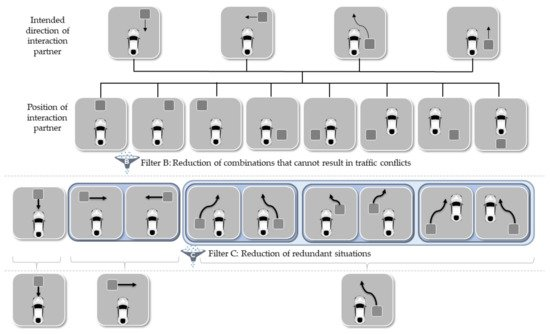
\includegraphics[width=14cm, height=13cm]{parking.jpg}
\bfseries\caption{\textbf{\textcolor{blue}{Intelegerea actiunilor care realizeaza salturile/mutarile masinilor}}}
\end{figure}

\vspace{3mm}

\newpage
	\begin{center}
	    \textcolor{blue}{\section{\bfseries\scshape\textcolor{blue}{Pseudo-codul algoritmilor propusi}}}
	   \vspace{10mm}
	\end{center}
\quad Algoritmii pe care i-am folosit pentru aceasta problema sunt divizati in mai multe functii in clasa numita m\_Vehicle care mosteneste clasa din fisierul search.py, Problem. La baza rezolvarii acestei probleme am folosit ca algoritmi de cautare, best first search, A* search, folosindu-ma si de distanta Manhattan, pentru a determina costul exact al deplasarii masinilor din starea initiala catre starea finala sau obiectiv.
\newline \\
Pseudo-codul algoritmilor implementati va fi prezentat mai jos, atat pentru algoritmii de cautare pe care ii folosesc, cat si pseudo-codul pentru fiecare functie implementat in cadrul rezolvarii temei de casa: \par
\vspace{5mm}
\quad 
\begin{center}
\begin{tabbing}
\large
\indent\textbf{\textcolor{blue}{func}}\=\textbf{\textcolor{blue}{tion}}
\textsc{\bfseries{BEST$\_$FIRST$\_$SEARCH}}{ ($problem,f$)}\ \textbf{returns} a solution node or none\\\\ 
\bfseries{1.}\indent \> $node \leftarrow$ a node with STATE = $problem.$INITIAL , PATH-COST = 0\\
\bfseries{2.}\indent \> $frontier \leftarrow $ a priority queue ordered by $f$\\
\bfseries{3.}\indent \> $explored  \leftarrow $ a lookup table, with one entry with key $problem.$INITIAL and value $node$\\
\bfseries{4.}\indent\>\textbf{while not} IS-EMPTY  \= $( frontier )$ \textbf{ do}\\
\bfseries{5.}\indent\> \ $node \leftarrow $POP($frontier$)\\
\bfseries{6.}\indent\>     \ \textbf{if } \= $problem.$IS-GOAL-Test( $node.$STATE ) \textbf{then}\\
\bfseries{7.}\indent\>   \>\textbf{return} $node$\\
\bfseries{8.}\indent\>      \textbf{end if}\\
\bfseries{9.}\indent\> \textbf{for each } $child$ \textbf{ in } EXPAND( $problem \ , \ node$ )\\
\bfseries{10.}\indent\>     \ \textbf{if } \= $child.$STATE \textbf{ is not } in $explored$ \textbf{and} $child$ \textbf{is not} in $frontier$\\ \indent\>     \> \ \textbf{or} $child.$PATH-COST $<$ $explored\ [child.STATE].PATH-COST$ \textbf{then}\\
\bfseries{11.}\indent\> \> $explored \ [child.STATE] \leftarrow child$\\
\bfseries{12.}\indent\> \> \textbf{add} $child$ \textbf{to} $frontier$\\
\bfseries{13.}\indent\>     \ \textbf{end if }\\
\bfseries{14.}\indent\> \textbf{end for}\\
\bfseries{15.}\indent\>\textbf{return} $none$\\\\
\indent\textbf{\textcolor{blue}{end }}\=\textbf{\textcolor{blue}{function}}
\end{tabbing}
\end{center}
\quad Denumirile variabileleor in Python, cat si implementarea difera din punct de vedere al sintaxei comparativ cu algoritmul in pseudo-cod, deoarece am incercat sa scriu algoritmii in pseudo-cod cat mai simplu si concins pentru a fi cititi si intelesi mai usor, implementarile din Python fiind adaptate in functie de fiecare algoritm in parte.\\ Specific faptul ca functiile de cautare fac parte din framework-ul aferent laboratorului 5.\par
\par
\begin{figure}
    \centering
    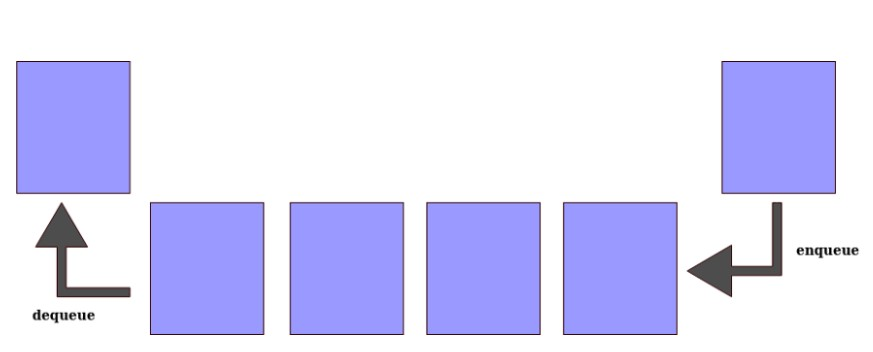
\includegraphics[width=15cm]{queue-diagram.jpg}
    \bfseries\caption{\textbf{\textcolor{blue}{O coada care urmareste nodurile urmatoare pentru a fi vizitate in continuare}}}
    \vspace{5mm}
\end{figure}
\quad
\begin{center}
\begin{tabbing}
\large
\indent\textbf{\textcolor{blue}{func}}\=\textbf{\textcolor{blue}{tion}}
\textsc{\bfseries{astar$\_$search}}{ ($node$)}\\\\
\bfseries{1.}\indent \> a priority queue with
priorities having as a function of cost on f (n) \\
\bfseries{2.}\indent \>\textbf{while} \= $ the\ destination\ node\ has\ not\ been\ reached $ \textbf{ do}\\
\bfseries{3.}\indent \> consider the $node$ with the lowest f score \textbf{in} the open list\\
\bfseries{4.}\indent\>   \> \textbf{if} \= this $node$ is our destination $node$ \textbf{then}\\
\bfseries{5.}\indent\>    \>  \>\textbf{return } finished\\
\bfseries{6.}\indent\>    \> \textbf{end if}\\
\bfseries{7.}\indent\>    \> \textbf{else }\\
\bfseries{8.}\indent\>    \> \> put the current $node$ in the closed list\\
\bfseries{9.}\indent\>    \> \>\textbf{for each} \= neighbor of the current node \\
\bfseries{10.}\indent\>   \>\>\>\textbf{if} \= neighbor has lower g value then current and is in the closed list \textbf{then}\\
\bfseries{11.}\indent\>   \>\>\>\> replace the neighbor with the new, lower g value\\
\bfseries{12.}\indent\>   \>\>\>\> current $node$ is now the neighbor's parent\\
\bfseries{13.}\indent\>   \>\>\>\textbf{end if}\\
\bfseries{14.}\indent\>   \>\>\>\textbf{else if} \= current g value is lower and this neighbor is in the open list \textbf{then}\\
\bfseries{15.}\indent\>    \>\>\>\>replace the neighbor with the new, lower, g value\\
\bfseries{16.}\indent\>     \>\>\>\>change the neighbor's parent to our current $node$\\
\bfseries{17.}\indent\>   \>\>\>\textbf{end else if}\\
\bfseries{18.}\indent\>   \>\>\>\textbf{else if} this neighbor is not in both list \textbf{then}\\
\bfseries{19.}\indent\>     \>\>\>\>\textbf{add} it to the open list and set its g\\
\bfseries{20.}\indent\>   \>\>\>\textbf{end else if}\\
\bfseries{21.}\indent\>    \> \>\textbf{end for}\\
\bfseries{22.}\indent \>\textbf{end while}\\\\
\indent\textbf{\textcolor{blue}{end }}\=\textbf{\textcolor{blue}{function}}
\end{tabbing}
\end{center}

\newpage
\begin{figure}
\sffamily
\quad Putem lua in considerare o retea 2D care are mai multe obstacole si pornim de la o celula sursa (colorata rosu) pentru a ajunge la o celula obiectiv (colorata verde).  Vrem sa atingem celula obiectiv (daca este posibil) pornind din celula de pornire cat mai repede posibil. \par
\newpage
  \vspace{7mm}
  \centering
  \begin{itemize}
     \item \textcolor{red}{\bfseries punctul rosu} = celula sursa
     \item \textcolor{green}{\bfseries punctul verde} = celula tinta
     \item \textcolor{black}{\bfseries patratele cu negru} = obstacole
 \end{itemize}
   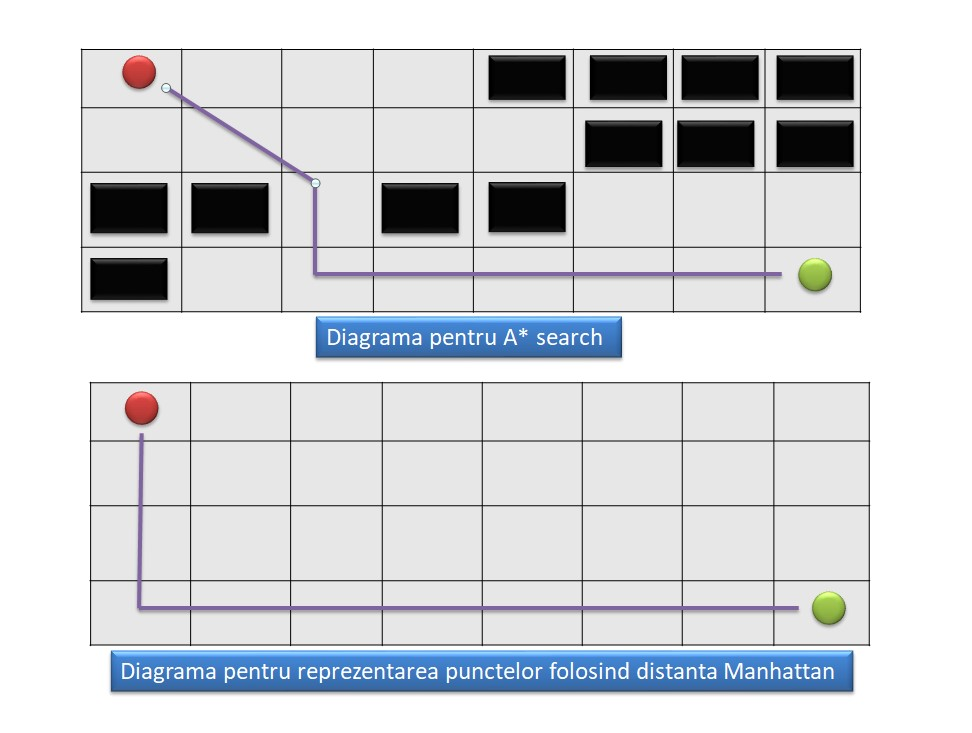
\includegraphics[width=13cm]{diagrame.jpg}
  \bfseries\caption{\textbf{\textcolor{blue}{Diagrame pentru o mai usoara abordare a problemei }}}
  \vspace{2cm}
  \quad \textbf{\textcolor{red}{\\ Observatie : }}Atasez mai jos link catre site-ul de unde m-am documentat, specific ca diagramele atasate mai sus au fost realizate in PowerPoint.\\
  \bfseries{\textcolor{blue}{\url{https://www.geeksforgeeks.org/a-search-algorithm/}}}
\end{figure}

\vspace{10mm}
\quad Am ales BEST-FIRST-SEARCH si A* search pentru a putea realiza un grafic compartiv pentru cei doi algoritmi in functie de costul caii, starea initiala, starea finala si in functie de actiunile executate de fiecare vehicul. Am observat ca best-first-search este mult mai optim din punct de vedere al timpului de executie decat A* search.\\ Dar ambii algoritmi fac parte din categoria algoritmilor "cautare intai-cel-mai-bun". Mai multe detalii vor fi precizate in sectiunea rezumatul rezultatelor.
\newline \\ 
Mai jos voi descrie pseudocod-ul pentru fiecare functie implementata in modulul implementation.py.\par

\vspace{5mm}
\begin{center}
\begin{tabbing}
\large
\indent\textbf{\textcolor{blue}{func}}\=\textbf{\textcolor{blue}{tion}}
\textsc{\bfseries{manhtDistance}}{($self,node$)}\textbf{ returns} the sum off all Manhattan distances\\\\ 
\bfseries{1.}\indent \> $node \leftarrow $ represents the state of a certain vehicle represented as a node\\ 
\bfseries{2.}\indent \> $manhattanDistance \leftarrow$ $sum(abs(s-g)*2\ for(s,g) \ in \ zip(node.state,self.goal))$ \\
\bfseries{3.}\indent \> \textbf{return}\ $ manhattanDistance$\\\\
\indent\textbf{\textcolor{blue}{end }}\=\textbf{\textcolor{blue}{function}}
\end{tabbing}
\end{center}

\quad Presupunem ca exista o singura masina care porneste de la  (\emph i, 1) si ca problema ar fi mutarea masinii respective pana la locatia sa.\\\\
Pornind de la formula distantei Manhattan, adica \(h_i\) = \( |x_1-x_2|+|y_1-y_2|\) pentru doua puncte din plan, $p_1 = (x_1, y_1)$ si $p_2 = (x_2, y_2)$, putem face afirmatia ca in cazul problemei noastre \\ \(h_i\) = |(\(\emph m - \emph i + 1\)) - \(x_i\)|+\(|\emph m\ - \) \(y_i\)| pentru a determina costul exact al deplasarii masinii catre obiectiv, iar scopul nostru este sa mutam toate masinile pe randul de sus, dar in ordine inversa astfel incat masina care porneste din celula (\emph i, 1) sa ajunga
in celula (\(\emph m - \emph i + 1, \emph m \)).\\\\
Daca ar exista alte masini in celula respectiva, aceasta nu ar mai fi neaparat o euristica admisibila, deoarece orice masina ar putea sa sara peste alte masini permitandu-i sa ajunga la obiectiv in mai putini pasi decat daca folosim distanta Manhattan. Si cunoastem faptul ca o functie euristica este admisibila daca poate sa estimeze in mod eficient distanta reala dintre un nod \emph n si nodul final, obiectiv. \\\\ Aceasta functie returneaza suma tuturor distantelor de la starea initiala la starea finala, fiind si functia care este folosita ca euristica pentru problema cautarii. Folosim distanta Manhattan deoarece ne ofera cel mai admisibil rezultat pentru aceasta problema, dar nu intocmai cel mai optim din punct de vedere al resurselor.\\ \par
\vspace{6mm}

\newpage
\quad Mai jos este prezentat pseudo-codul pentru crearea \textbf{starii initiale si scop}. \\
Initializam problema cu dimensiunea parcarii, starea initială si starea obiectivului.\par
\vspace{6mm}
\begin{center}
\begin{tabbing}
\large
\indent\textbf{\textcolor{blue}{func}}\=\textbf{\textcolor{blue}{tion}}
\textsc{\bfseries{\_\_init\_\_}}{($self, parking\_size, stare\_initiala, stare\_finala$)}\\\\ 
\bfseries{1.}\indent \> $self.parking\_size \leftarrow$ $parking\_size$ \\\
\bfseries{2.}\indent \> $self.initial \leftarrow$ $stare\_initiala$ \\\
\bfseries{3.}\indent \> $self.goal \leftarrow$ $stare\_finala$\\\
\bfseries{4.}\indent \> $self.mutare\_masina \leftarrow$ $-1$ \\\
\bfseries{5.}\indent \>\bfseries Problem.\_\_init\_\_{$self, initial, goal$}\\\\
\indent\textbf{\textcolor{blue}{end }}\=\textbf{\textcolor{blue}{function}}
\end{tabbing}
\end{center}
\quad Masinile sunt reprezentate in figura 1  pentru a le putea diferentia si ordona in sens invers pe ultima linie. \\
 Numarul de moduri de a plasa \emph m masini distincte in \emph m × \emph m celule este : \par
 \vspace{6mm}
\(m^2\)(\(m^2\) - 1 ) $\dots$ (\(m^2\) - m + 1) \(\in\) O (\(n^2\*^n\)) \\\\
\newline
\quad Fiecare masina are cel mult 5 miscari posibile din orice pozitie (UP, DOWN, LEFT, RIGHT si STAY). Retinem ca daca fiecare masina are o celula 3 x 3 de spatiu gol in jurul ei rezulta ca toate cele cinci miscari sunt posibile pentru fiecare masina si acestea vor avea ca rezultat configuratii unice (deoarece masinile nu vor interactiona).\\
Cand m este suficient de mare avem suficiente celule de 3 x 3 pentru a sustine toate masinile posibile.\\\\
\textbf{\textcolor{red}{Exemplu: \\}} 
Luam in considerare cand m = 12. Exista 16 celule 3 x 3 rezulta ca putem sustine toate cele 12 masini si chiar urmatoarele doua pe masura ce marim dimensiunea celulei.\\
De fiecare data cand crestem m cu 3, putem sustine in mod clar cel putin doua
masini care depasesc dimensiunea parcarii. Daca masina \emph i se afla la destinatie, atunci valoarea euristica este 0, care reprezinta si  costul exact, rezulta, prin urmare, acesta este admisibil, altfel cand un vehicul efectueaza un salt peste alt vehicul, masina peste care sare nu poate fi la destinatie, ceea ce ar duce la o contradictie, astfel fiind dat masina care este sarita trebuie sa aiba cel putin un pas ramanand pana la destinatie. \\\\
\textbf{\textcolor{red}{Concluzia: \\}} 
Eliminam anumite actiuni in functie de pozitia in parcare a masinilor, spre exemplu sa nu faca miscari in afara matricei( parcarii ), sa nu faca salturi aiurea in afara matricei sau peste 2 masini.\\
Fiecare actiune executata de ficare vehicul implica un cost = 1, iar factorul de ramificare in cel mai rau caz este = $5^n$.\\
\par
\newpage
\begin{figure}
\sffamily
    \centering
    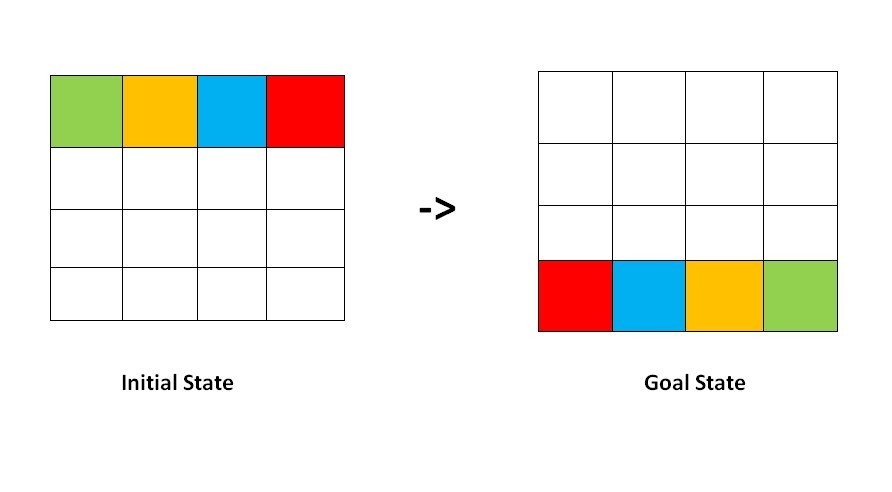
\includegraphics[width=16cm]{stare-initiala-si-obiectiv.jpg}\\[0.5cm]
    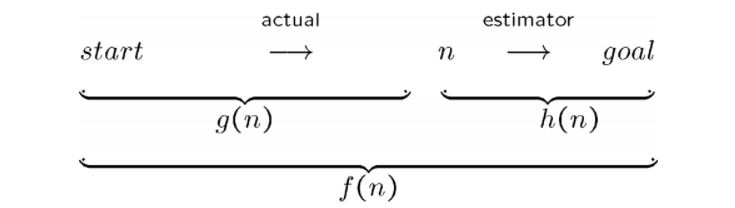
\includegraphics[width=15cm]{abordare-functie.JPG}
    \bfseries\caption{\textbf{\textcolor{blue}{Starea initiala si obiectivul }}}
\end{figure}
\newpage

\quad
\begin{center}
  \textbf{\textcolor{red}{initial state} :} configuratia initiala a masinilor in parcare.\\ 
  \textbf{\textcolor{red}{goal state} :} configuratia finala a masinilor in parcare.\par
  \quad \\ Scopul este sa mutam toate masinile pe randul de sus, dar in ordine inversa, astfel incat masina care porneste din celula (\emph i, 1) sa ajunga
  in celula (\(\emph m - \emph i + 1, \emph m \)).\par
\end{center}
\newpage
\quad Din cerinta problemei deducem faptul ca fiecare masina are cel mult 5 miscari posibile din orice pozitie (SUS, JOS, STANGA, DREAPTA si STAY) plus salturile/sariturile pe care le poate executa fiecare vehicul. \\ Adica fiecare vehicul poate executa mai multe actiuni pentru a atinge starea finala intr-un mod admisibil, in functie de locatia sa in parcare sau de pozitia celorlalte vehicule, acesta se poate deplasa inainte, inapoi, la stanga, la dreapta, respectiv poate executa salturi peste celelalte vehicule(daca este permis), sau poate sta pe loc in celula pe care deja o ocupa.\\ Calculam urmatoarea mutare a vehicului iar, daca vehiculul dinainte a executat o mutare atunci pozitia vehicului va deveni 0 si va incepe din nou cu primul vehicul, altfel trecem la pozitia urmatorului vehicul. \\\par
\quad Verificam directiile pe care vehiculul nostru le poate realiza, conform parcarii, apo verificam actiunile pe care le poate face vehiculul nostru, conform celorlalte vehicule si eliminam anumite actiuni in functie de pozitia vehiculelor.\\ Returnam actiunile care pot fi executate in starea data, iar rezultatul este o lista, deoarece exista doar cinci actiuni posibile, plus salturile/sariturile pe care le poate executa fiecare vehicul.\\ Exista si anumite reguli, cum ar fi: \\
\begin{itemize}
    \item 2 vehicule nu poate imparti acelasi loc de parcare, deci daca un vehicul
    este deasupra altui vehicul, acest vehicul nu poate sa coboare, deci
    actiunile descendente vor fi eliminate din lista cu actiuni posibile.
    \item cand un vehicul nu poate iesi in afara parcarii, asta inseamna ca atunci cand este plasat pe primul rand, nu poate merge in sus, astfel incat actiunile sus vor fi eliminate din lista actiunilor posibile.
\end{itemize}
Aceasta functie va fi utilizata pentru fiecare vehicul, tinandu-se cont de reguli, respectiv cazurile in care se afla fiecare vehicul.\par
Mai jos este prezentat pseudo-codul pentru implementarea functiei care verifica directiile pe care vehiculul nostru le poate realiza, conform parcarii. \\
\begin{center}
\begin{tabbing}
\large
\indent\textbf{\textcolor{blue}{func}}\=\textbf{\textcolor{blue}{tion}}
\textsc{\bfseries actions}\ {($self,stare$)}\ \textbf{returns} an action\\\\
\bfseries{1.}\indent\>\textbf{if } \=$self.mutare\_masina$ $==$ $self.parking\_size - 1$ \textbf{then} \\
\bfseries{2.}\indent\>         \> $self.mutare\_masina \leftarrow$ 0 \\
\bfseries{3.}\indent\>\textbf{else}\\
\bfseries{4.}\indent\>         \>$self.mutare\_masina \leftarrow$ $self.mutare\_masina + 1$\\
\bfseries{5.}\indent\>\textbf{end if}\\
\bfseries{6.}\indent\>\textbf{ListaActiunilorPosibile} $\leftarrow$ $list[ 'SUS' + str( self.mutare\_masina ) ,\ 'JOS' + str( self.mutare\_masina ) , $\\\indent\> $ 'STANGA' + str( self.mutare\_masina ) ,\ 'DREAPTA' + str( self.mutare\_masina ) , $ \\ \indent \> $ 'STAY' + str( self.mutare\_masina ),\ 'SARITURA\ STANGA' + str( self.mutare\_masina ),$\\\indent\>$'SARITURA\ DREAPTA' + str( self.mutare\_masina ),\ 'SARITURA\ INAINTE' $\\\indent\>$+ str( self.mutare\_masina ),\ 'SARITURA\ INAPOI' + str( self.mutare\_masina )] $\\
\bfseries{7.}\indent\>\textbf{locatia1} $\leftarrow$ $state[self.mutare\_masina]$\\
\bfseries{8.}\indent\>\textbf{if } \=$locatia1$ $<$ $self.parking\_size$ \textbf{ then}\\
\bfseries{9.}\indent\>       \>\textbf{if } \=$'SUS'$ $+$ $str(self.mutare\_masina) \ in \ $ \textbf{ListaActiunilorPosibile} \textbf{ then} \\
\bfseries{10.}\indent          \> \> \>\textbf{ListaActiunilorPosibile}.$remove('SUS'$ $+$ $str(self.mutare\_masina))$\\
\bfseries{11.}\indent\>        \>\textbf{end if}\\
\bfseries{12.}\indent\>\textbf{end if}\\
\bfseries{13.}\indent\> \textbf{if } \=$locatia1$ $>=$ $self.parking\_size*(self.parking\_size-1)$ \textbf{ then}\\
\bfseries{14.}\indent\>       \>\textbf{if } \=$'JOS'$ $+$ $str(self.mutare\_masina) \ in \ $ \textbf{ListaActiunilorPosibile} \textbf{ then} \\
\bfseries{15.}\indent          \> \> \>\textbf{ListaActiunilorPosibile}.$remove('JOS'$ $+$ $str(self.mutare\_masina))$\\
\bfseries{16.}\indent\>        \>\textbf{end if}\\
\bfseries{17.}\indent\>\textbf{end if}\\
\bfseries{18.}\indent\>\textbf{if } \=$locatia1$ \textbf{ modulo } $self.parking\_size$ $==$ 0 \textbf{ then}\\
\bfseries{19.}\indent\>       \>\textbf{if } \=$'STANGA'$ $+$ $str(self.mutare\_masina) \ in \ $ \textbf{ListaActiunilorPosibile} \textbf{ then} \\
\bfseries{20.}\indent          \> \> \>\textbf{ListaActiunilorPosibile}.$remove('STANGA'$ $+$ $str(self.mutare\_masina))$\\
\bfseries{21.}\indent\>        \>\textbf{end if}\\
\bfseries{22.}\indent\>\textbf{end if}\\
\bfseries{23.}\indent\>\textbf{if } \=$locatia1$ \textbf{ modulo } $self.parking\_size$ $==$ $self.parking\_size - 1$ \textbf{ then}\\
\bfseries{24.}\indent\>       \>\textbf{if } \=$'DREAPTA'$ $+$ $str(self.mutare\_masina) \ in \ $ \textbf{ListaActiunilorPosibile} \textbf{ then} \\
\bfseries{25.}\indent          \> \> \>\textbf{ListaActiunilorPosibile}.$remove('DREAPTA'$ $+$ $str(self.mutare\_masina))$\\
\bfseries{26.}\indent\>        \>\textbf{end if}\\
\bfseries{27.}\indent\>\textbf{end if}\\
\bfseries{28.}\indent\>\textbf{if } \=$locatia1$ \textbf{ modulo } $self.parking\_size$ $<=$ $1$ \textbf{ then}\\
\bfseries{29.}\indent\>       \>\textbf{if } \=$'SARITURA\ STANGA'$ $+$ $str(self.mutare\_masina) \ in \ $ \textbf{ListaActiunilorPosibile} \textbf{ then} \\
\bfseries{30.}\indent          \> \> \>\textbf{ListaActiunilorPosibile}.$remove('SARITURA\ STANGA'$ $+$ $str(self.mutare\_masina))$\\
\bfseries{31.}\indent\>        \>\textbf{end if}\\
\bfseries{32.}\indent\>\textbf{end if}\\
\bfseries{33.}\indent\>\textbf{if } \=$locatia1$ \textbf{ modulo } $self.parking\_size$ $>=$ $self.parking\_size-2$ \textbf{ then}\\
\bfseries{34.}\indent\>       \>\textbf{if } \=$'SARITURA\ DREAPTA'$ $+$ $str(self.mutare\_masina) \ in \ $ \textbf{ListaActiunilorPosibile} \textbf{ then} \\
\bfseries{35.}\indent          \> \> \>\textbf{ListaActiunilorPosibile}.$remove('SARITURA\ DREAPTA'$ $+$ $str(self.mutare\_masina))$\\
\bfseries{36.}\indent\>        \>\textbf{end if}\\
\bfseries{37.}\indent\>\textbf{end if}\\
\bfseries{38.}\indent\>\textbf{if } \=$locatia1$ $<$ $self.parking\_size*2$ \textbf{ then}\\
\bfseries{39.}\indent\>       \>\textbf{if } \=$'SARITURA\ INAINTE'$ $+$ $str(self.mutare\_masina) \ in \ $ \textbf{ListaActiunilorPosibile} \textbf{ then} \\
\bfseries{40.}\indent          \> \> \>\textbf{ListaActiunilorPosibile}.$remove('SARITURA\ INAINTE'$ $+$ $str(self.mutare\_masina))$\\
\bfseries{41.}\indent\>        \>\textbf{end if}\\
\bfseries{42.}\indent\>\textbf{end if}\\
\bfseries{43.}\indent\>\textbf{if } \=$locatia1$ $>$ $self.parking\_size^2-2*self.parking\_size-1$  \textbf{ then}\\
\bfseries{44.}\indent\>       \>\textbf{if } \=$'SARITURA\ INAPOI'$ $+$ $str(self.mutare\_masina) \ in \ $ \textbf{ListaActiunilorPosibile} \textbf{ then} \\
\bfseries{45.}\indent          \> \> \>\textbf{ListaActiunilorPosibile}.$remove('SARITURA\ INAPOI'$ $+$ $str(self.mutare\_masina))$\\
\bfseries{46.}\indent\>        \>\textbf{end if}\\
\bfseries{47.}\indent\>\textbf{end if}\\
\bfseries{48.}\indent\>idx $\leftarrow$ 0\\ 
\bfseries{49.}\indent\> \textbf{while} idx  $<$ \= $self.parking\_size$ \textbf{ do}\\
\bfseries{50.}\indent\> \ {locatia2 } == \=$stare[idx]$  \\
\bfseries{51.}\indent\> \textbf{if } idx  $\neq$ \= $self.mutare\_masina$ \textbf{ then}\\
\bfseries{52.}\indent\>       \>\textbf{if } \=$locatia1$ $-$ $self.parking\_size \ == \ $ $ locatia2$ \textbf{ then} \\
\bfseries{53.}\indent\>       \>\>\textbf{if } \=$'SUS'$ $+$ $str(self.mutare\_masina) \ in \ $ \textbf{ListaActiunilorPosibile} \textbf{ then} \\
\bfseries{54.}\indent          \> \> \> \>\textbf{ListaActiunilorPosibile}.$remove('SUS'$ $+$ $str(self.mutare\_masina))$\\
\bfseries{55.}\indent          \> \>  \>\textbf{end if}\\
\bfseries{56.}\indent\>        \>\textbf{end if}\\
\bfseries{57.}\indent\>       \>\textbf{if } \=$locatia1$ $+$ $self.parking\_size \ == \ $ $ locatia2$ \textbf{ then} \\
\bfseries{58.}\indent\>       \>\>\textbf{if } \=$'JOS'$ $+$ $str(self.mutare\_masina) \ in \ $ \textbf{ListaActiunilorPosibile} \textbf{ then} \\
\bfseries{59.}\indent          \> \> \> \>\textbf{ListaActiunilorPosibile}.$remove('JOS'$ $+$ $str(self.mutare\_masina))$\\
\bfseries{60.}\indent          \> \>  \>\textbf{end if}\\
\bfseries{61.}\indent\>        \>\textbf{end if}\\
\bfseries{62.}\indent\>       \>\textbf{if } \=$locatia1$ $-$ $ 1 \ == \ $ $ locatia2$ \textbf{ then} \\
\bfseries{63.}\indent\>       \>\>\textbf{if } \=$'STANGA'$ $+$ $str(self.mutare\_masina) \ in \ $ \textbf{ListaActiunilorPosibile} \textbf{ then} \\
\bfseries{64.}\indent          \> \> \> \>\textbf{ListaActiunilorPosibile}.$remove('STANGA'$ $+$ $str(self.mutare\_masina))$\\
\bfseries{65.}\indent          \> \>  \>\textbf{end if}\\
\bfseries{66.}\indent\>        \>\textbf{end if}\\
\bfseries{67.}\indent\>       \>\textbf{if } \=$locatia1$ $+$ $ 1 \ == \ $ $ locatia2$ \textbf{ then} \\
\bfseries{68.}\indent\>       \>\>\textbf{if } \=$'DREAPTA'$ $+$ $str(self.mutare\_masina) \ in \ $ \textbf{ListaActiunilorPosibile} \textbf{ then} \\
\bfseries{69.}\indent          \> \> \> \>\textbf{ListaActiunilorPosibile}.$remove('DREAPTA'$ $+$ $str(self.mutare\_masina))$\\
\bfseries{70.}\indent          \> \>  \>\textbf{end if}\\
\bfseries{71.}\indent\>        \>\textbf{end if}\\
\bfseries{72.}\indent\>       \>\textbf{if } \=$locatia1$ $-$ $ 2 \ == \ $ $ locatia2$ \textbf{ then} \\
\bfseries{73.}\indent\>       \>\>\textbf{if } \=$'SARITURA\ STANGA'$ $+$ $str(self.mutare\_masina) \ in \ $ \textbf{ListaActiunilorPosibile} \textbf{ then} \\
\bfseries{74.}\indent          \> \> \> \>\textbf{ListaActiunilorPosibile}.$remove('SARITURA\ STANGA'$ $+$ $str(self.mutare\_masina))$\\
\bfseries{75.}\indent          \> \>  \>\textbf{end if}\\
\bfseries{76.}\indent\>        \>\textbf{end if}\\
\bfseries{77.}\indent\>       \>\textbf{if } \=$locatia1$ $+$ $ 2 \ == \ $ $ locatia2$ \textbf{ then} \\
\bfseries{78.}\indent\>       \>\>\textbf{if } \=$'SARITURA\ DREAPTA'$ $+$ $str(self.mutare\_masina) \ in \ $ \textbf{ListaActiunilorPosibile} \textbf{ then} \\
\bfseries{79.}\indent          \> \> \> \>\textbf{ListaActiunilorPosibile}.$remove('SARITURA\ DREAPTA'$ $+$ $str(self.mutare\_masina))$\\
\bfseries{80.}\indent          \> \>  \>\textbf{end if}\\
\bfseries{81.}\indent\>        \>\textbf{end if}\\
\bfseries{82.}\indent\>       \>\textbf{if } \=$locatia1$ $-$ $ 2*self.parking\_size \ == \ $ $ locatia2$ \textbf{ then} \\
\bfseries{83.}\indent\>       \>\>\textbf{if } \=$'SARITURA\ INAINTE'$ $+$ $str(self.mutare\_masina) \ in \ $ \textbf{ListaActiunilorPosibile} \textbf{ then} \\
\bfseries{84.}\indent          \> \> \> \>\textbf{ListaActiunilorPosibile}.$remove('SARITURA\ INAINTE'$ $+$ $str(self.mutare\_masina))$\\
\bfseries{85.}\indent          \> \>  \>\textbf{end if}\\
\bfseries{86.}\indent\>        \>\textbf{end if}\\
\bfseries{87.}\indent\>       \>\textbf{if } \=$locatia1$ $+$ $ 2*self.parking\_size \ == \ $ $ locatia2$ \textbf{ then} \\
\bfseries{88.}\indent\>       \>\>\textbf{if } \=$'SARITURA\ INAPOI'$ $+$ $str(self.mutare\_masina) \ in \ $ \textbf{ListaActiunilorPosibile} \textbf{ then} \\
\bfseries{89.}\indent          \> \> \> \>\textbf{ListaActiunilorPosibile}.$remove('SARITURA\ INAPOI'$ $+$ $str(self.mutare\_masina))$\\
\bfseries{90.}\indent          \> \>  \>\textbf{end if}\\
\bfseries{91.}\indent\>        \>\textbf{end if}\\
\bfseries{92.}\indent\>\textbf{end if }\\
\bfseries{93.}\indent\>$idx \leftarrow idx + 1$ \\
\bfseries{94.}\indent\>\textbf{end while }\\
\bfseries{95.}\indent\>\textbf{return ListaActiunilorPosibile }\\
\indent\textbf{\textcolor{blue}{end }}\=\textbf{\textcolor{blue}{function}}
\end{tabbing}
\end{center}
\subsection*{\textcolor{red}{Observatie}}
\quad Din punct de vedere al sintaxei si pentru a optimiza algoritmul, am modificat liniile 52-87 de mai sus in implementarea din Python, punand cele 2 instructiuni if intr-o singura instructiune if, folosind operatorul logic 'and', atat sintaxa de mai sus, cat si sintaxa modificata in Python returneaza acelasi rezultat, in cadrul pseudo-codului de mai sus nu am mai modificat sintaxa, m-am gandit la o imbunatatire a algoritmului in Python dupa ce scrisesem deja  pseudo-codul aici. \par
\vspace{10mm}
\newpage
\quad Avand in vedere starea si actiunea, revenim la o noua stare care reprezinta rezultatul actiunii finale. Actiunea se presupune ca este o actiune valida. \\ 
Mai jos este prezentat pseudo-codul pentru implementarea functiei care returneaza noua stare calculata in functie de actiunile posibile. Starea noua reprezinta pozitia vehicului \emph{i} si actiunea pe care o executa vehiculul. \par
\vspace{10mm}
\begin{center}
\begin{tabbing}
\large
\indent\textbf{\textcolor{blue}{func}}\=\textbf{\textcolor{blue}{tion}}
\textsc{\bfseries result}\ {($self,stare, actiune$)}\textbf{ returns} the new state calculated according to the possible actions\\\\
\bfseries{1.}\indent\>$locatia1 \leftarrow stare[self.mutare\_masina]$\\
\bfseries{2.}\indent\>$noua\_stare \leftarrow list[stare]$\\
\bfseries{3.}\indent\>\textbf{delta} $\leftarrow$ $list[ 'SUS' + str( self.mutare\_masina ):-self.parking\_size ,$\\\indent\> $ 'JOS' + str( self.mutare\_masina ):+self.parking\_size , $\\\indent\> $ 'STANGA' + str( self.mutare\_masina ):-1 ,$\\\indent\> $ 'DREAPTA' + str( self.mutare\_masina ):+1 , $ \\ \indent \> $ 'STAY' + str( self.mutare\_masina ): 0, 'SARITURA\ STANGA' + str( self.mutare\_masina ): -2,$\\\indent\> $'SARITURA\ DREAPTA' + str( self.mutare\_masina ): +2,$\\\indent\>$'SARITURA\ INAINTE' + str( self.mutare\_masina ): -2*self.parking\_size,$\\\indent\>$'SARITURA\ INAPOI' + str( self.mutare\_masina ): +2*self.parking\_size \ ] $\\
\bfseries{4.}\indent \>$noua\_stare[self.mutare\_masina] \leftarrow locatia1 + $\textbf{delta}[actiune]\\
\bfseries{5.}\indent \> \textbf{return }$tuple(noua\_stare)$\\\\
\indent\textbf{\textcolor{blue}{end }}\=\textbf{\textcolor{blue}{function}}
\end{tabbing}
\end{center}
\vspace{7mm}
\quad \par Am exprimat delta ca actiune pe care o poate executa un vehicul, adica retine rezultatul pentru fiecare actiune. Apoi returnam rezultatul actiunii ca fiind un tuplu.\\ Ca idee, avem in vedere o stare si returnam true daca starea respectiva este o stare a obiectivului nostru sau false, altfel.\\
\quad Pentru calcularea modificarii pe care o actiune o face asupra starii avem mai multe cazuri:\\\\
\textcolor{blue}{\bfseries$-$} daca actiunea va fi „SUS”, aceasta va scadea valoarea variabilei parking$\_$size din starea actuala a vehiculului;\\
\textcolor{blue}{\bfseries$-$} daca actiunea va fi „JOS”, adauga aceasta valoare la starea actuala;\\
\textcolor{blue}{\bfseries$-$} daca actiunea este la „DREAPTA” adauga 1 la starea actuala;\\
\textcolor{blue}{\bfseries$-$} daca actiunea este la „STANGA” scade 1;\\
\textcolor{blue}{\bfseries$-$} iar daca actiunea este „STAY” nu face nimic, deoarece vehiculul nu se misca, sta pe loc.\\\\
Tot aici, au fost luate in calcul si cazurile cand un vehicul poate efectua o saritura la dreapta, la stanga, inainte sau inapoi peste un alt vehicul, astfel incat obiectivul sa fie indeplinit intr-un mod admisibil, tinandu-se cont de locatia vehicului respectiv in parcare sau de pozitia celorlalte vehicule, indeplinind cazurile enumerate mai sus.
\newpage
\begin{center}
     \textcolor{blue}{\section{\bfseries\scshape\textcolor{blue}{Date experimentale}}}
\end{center}
\quad 
Pseudo-codul algoritmiilor care ne genereaza formatul datelor de intrare este prezentat mai jos :
\par
\vspace{15mm}
\begin{center}
\begin{tabbing}
\large
\indent\textbf{\textcolor{blue}{func}}\=\textbf{\textcolor{blue}{tion}}
\textsc{\bfseries{generare$\_$dimensiune$\_$parcare}}\\\\
1.\indent \> \textbf{return} $random.randint(1,7)$\\\\
\indent\textbf{\textcolor{blue}{end }}\=\textbf{\textcolor{blue}{function}}
\end{tabbing}
\end{center}
\vspace{1cm}
\begin{center}
\begin{tabbing}
\large
\indent\textbf{\textcolor{blue}{func}}\=\textbf{\textcolor{blue}{tion}}
\textsc{\bfseries{generare$\_$stare$\_$initiala}}\ {($dimensiune$)}\\\\
\bfseries{1.}\indent \> stare$\_$initiala $\leftarrow$ tuple()\\
\bfseries{2.}\indent \> idx $\leftarrow$ 0 \\
\bfseries{3.}\indent\> \textbf{while} idx  $<$ \= $dimensiune$ \textbf{ do}\\
\bfseries{4.}\indent\>   \>stare$\_$initiala $\leftarrow$stare$\_$initiala$+$ $tuple([dimensiune*idx])$\\
\bfseries{5.}\indent\>   \>idx $\leftarrow$ idx $+$ 1\\
\bfseries{6.}\indent\>\textbf{end while}\\
\bfseries{7.}\indent\> \textbf{return} stare$\_$initiala\\\\
\indent\textbf{\textcolor{blue}{end }}\=\textbf{\textcolor{blue}{function}}
\end{tabbing}
\end{center}
\vspace{1cm}
\begin{center}
\begin{tabbing}
\large
\indent\textbf{\textcolor{blue}{func}}\=\textbf{\textcolor{blue}{tion}}
\textsc{\bfseries{generare$\_$stare$\_$finala}}\ {($dimensiune$\ ,\ $stare\_initiala$)}\\\\
\bfseries{1.}\indent \> generare$\_$stare$\_$finala $\leftarrow$ tuple()\\
\bfseries{2.}\indent \> idx $\leftarrow$ 0 \\
\bfseries{3.}\indent\> \textbf{while} idx  $<$ \= $dimensiune$ \textbf{ do}\\
\bfseries{4.}\indent\>   \>stare$\_$finala $\leftarrow$ stare$\_$finala $+$ $tuple([(dimensiune^2)-stare\_initiala[idx]-1])$\\
\bfseries{5.}\indent\>   \>idx $\leftarrow$ idx $+$ 1\\
\bfseries{6.}\indent\>\textbf{end while}\\
\bfseries{7.}\indent\> \textbf{return} stare$\_$finala\\\\
\indent\textbf{\textcolor{blue}{end }}\=\textbf{\textcolor{blue}{function}}
\end{tabbing}
\end{center}

\newpage 
\vspace{5cm}
Folosim o metoda pentru generarea automata a datelor de intrare, astfel incat generam aleatoriu dimensiunea parcarii, starea initiala si cea finala in functie de dimensiunea parcarii. Mai jos descriu care este metoda pentru generare, de ce folosesc o metoda de generare random a datelor de intrare si care este intervalul de generare pentru datele de intrare.\\\\

Folosim functia \emph randint pentru a returna un numar intreg aleatoru situat in intervalul\\ (0, \emph randint$\_$max), unde randint$\_$max este valoarea maxima pe care o poate lua intervalul nostru generand aleatoriu toate valorile din intervalul respectiv. Cu ajutorul buclei \emph while putem specifica limita unei secvente de valori, astfel functiile pentru generarea starii initiale, cat si pentru generarea starii finale o sa returneze un numar aleatoru selectat din intervalul nostru, dar nu mai mare de valoarea limita pentru dimensiunea parcarii.\\\\

Generam random dimensiunea parcarii \emph m x \emph m. Returnam aleatoriu un numar cuprins intre 1 si 7. Cum limbajul Python este mai lent din punct de vedere a timpului de executie, folosim functiile deja scrise din modulele limbajului.\\\\ 

Generam starea initiala cu pozitia de pornire pentru fiecare vehicul, care este prima coloana a unei matrice, dar fiecare pozitie i, j din matrice este notata cu valori incepand de la 0 pana la dimensiunea parcarii astfel, daca i = 1 si j = 1, pozitia va fi 0; \ pentru i = 1 și j = 2, pozitia va fi 1 si asa mai departe pana la ultima pozitie, care va fi egal cu numarul variabilei parking\_size, adica dimensiunea parcarii.\\\\

Generam starea obiectivului, urmand aceeasi idee ca mai sus, dar folosind o o alta formula, deoarece fiecare vehicul trebuie sa ajunga la pozitia cu coordonatele 
(\emph m - \emph i + 1 , \emph m), asta inseamna ca trebuie sa ajunga pe randul de sus, dar în ordine inversa. In conformitate cu cele enumerate mai sus, putem argumenta faptul ca datele generate de algoritmul nostru prezentat sunt semnificative pentru testarea problemei din tema de casa.\\\\

Acesti algoritmi genereaza aleatoriu dimensiunea parcarii \emph m x \emph m , starea initiala si starea finala; dimensiunea parcarii fiind data aleatoriu intre 1 si 7, iar starea initiala, cat si cea finala au valorile generate in functie de dimensiunea parcarii. Cum intervalul de generare a datelor este cuprins intre (1,7), rezulta ca datele de intrare sunt admisibile, dar, doar pana la o dimensiunea de \emph 7 x \emph 7, deoarece doar intre aceste valori algoritmul ofera un raspuns.\\ Mai multe detalii despre rezultatele obtinute vor fi abordate in sectiunea rezumatul rezultatelor. 
\newpage
\begin{figure}
  \vspace{9mm}
  \centering
  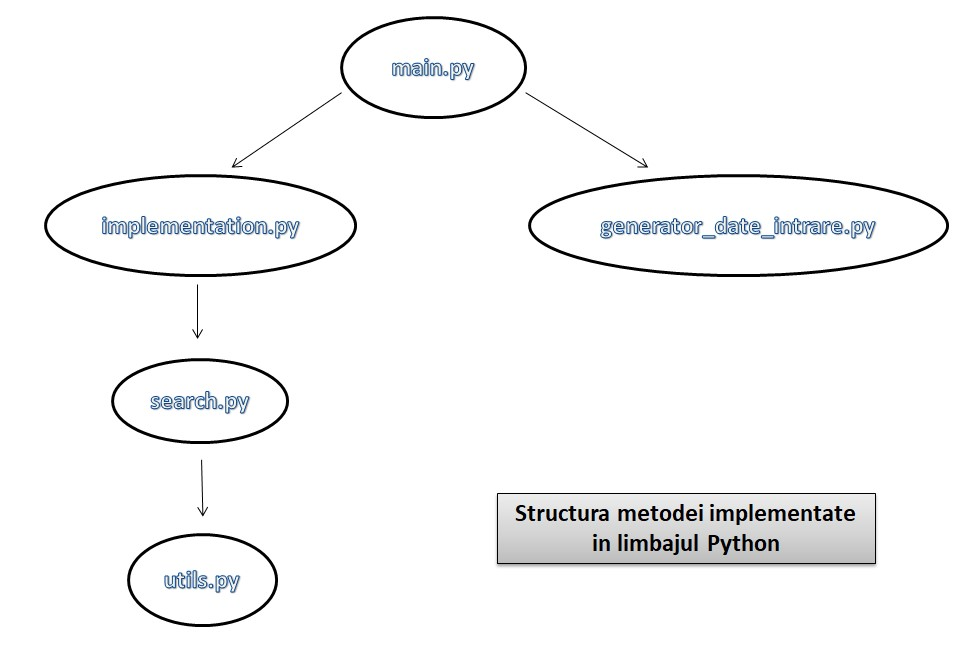
\includegraphics[width=15cm, height=15cm]{structuradenivelinalt.jpg}
  \bfseries\caption{\textbf{\textcolor{blue}{Structura de nivel inalt a aplicatiei}}}
\end{figure}

\newpage   
\begin{center}
     \textcolor{blue}{\section{\bfseries\scshape\textcolor{blue}{Proiectarea aplicatiei}}}
\end{center}
\vspace{7mm}
 \textcolor{blue}{\subsection{\itshape \textcolor{blue}{Structura de nivel inalt a aplicatiei }}}
\vspace{10mm}
\begin{flushleft}
\quad Aplicatia creata este organizata in module, fiecare modul continand functii particulare. Specific faptul ca pentru rezolvarea problemei din tema de casa am folosit framework-ul de la 15-puzzle problem din platforma de laborator 5, adaptand, testand si gasind o euristica aferent potrivita implementarii acestui assigment.\\
\vspace{2mm}
Astfel pentru rezolvarea problemei in limbajul Python, programul este divizat in mai multe fisiere.\\
Fiecare modul contine functii ce ajuta la rezolvarea problemei, importandu-le direct din fisierele dorite.  
Functiile programului sunt apelate in fisierul main.py, ce reprezinta fisierul principal ce ruleaza programul.\par 
\vspace{3mm}
\quad \textcolor{red}{\bfseries Structura acestuia arata in felul urmator :} \par
\end{flushleft}

\begin{itemize}
  \item  main.py $-$ fisierul principal ce ruleaza programul;
  \item implementation.py $-$ fisierul unde sunt definite actiunile in functie de  miscariile masinilor;
  \item generator\_date\_intrare.py $-$ fisier ce contine implementate functii pentru generare random a datelor de intrare;
  \item search.py $-$ fisier unde sunt apelate diverse functii de cautare;
  \item utils.py $-$ fisier ce ofera anumite utilitati pentru rezolvarea problemei;
\end{itemize}
\vspace{2mm}

\begin{flushleft}
\quad In fisierul generator\_date\_intrare gasim trei funtii implementate cu scopul de a genera random datele de intrare pentru dimensiunea parcarii, starea initiala si starea finala.  \\ 
\vspace{2mm}
Am folosit aceasta structura modulara pentru ca la final sa putem observa mai bine diferenta dintre rezultatul final, cat si timpul necesar rezolvari problemei pentru anumite date de intrare random. Pe urmatoarea pagina intalnim o diagrama realizata in PowerPoint pentru structura metodei implementate in limbajul Python.\par
\end{flushleft}
\newpage
\begin{flushleft}
    \textcolor{blue}{\subsection{\itshape \textcolor{blue}{Specificatia formatului datelor de intrare}}}
     \vspace{5mm}
\end{flushleft}

\begin{flushleft}
\quad Pentru generarea datelor de intrare, am creat un nou fisier numit generator$\_$date$\_$intrare.py care contine implementate 3 functii care calculeaza dimensiunea parcarii in mod aleatoriu si, de asemenea, calculeaza starea initiala si starea obiectivului conform unor reguli matematice. Acestea genereaza aleatoriu date de intrare relevante si netriviale pentru testarea algorimului.\\  \par
\vspace{2mm}
\quad Datele de intrare reprezinta dimensiunea unei parcari sau a unei matrice \emph m × \emph m, dimensiune ce este generata aleatoriu, iar \emph m reprezinta dimenisiunea matricei; in functie de dimensiunea matricei generam si numarul de masini.\\ \par 
\vspace{2mm}
\quad Fiecare element din matrice reprezinta o locatie in parcare si este reprezentat printr-un numar pozitiv si intreg semnificand cota locatiei respective in parcare.\\ \par
\vspace{2mm}
\quad Definim actiunile in functie de miscarile masinilor, adica calculam pentru fiecare stare care masina sa fie mutata pentru a putea muta doar o masina la un pas anume, tinand cont de specificatiile cerintei din tema de casa.\par
\end{flushleft}
\begin{flushleft}
    \textcolor{blue}{\subsection{\itshape \textcolor{blue}{Specificatia formatului datelor de iesire}}}
    \vspace{5mm}
\end{flushleft}
\begin{flushleft}
\quad Datele de iesire sunt generate de functia astar search din fisierul search.py. Aceasta functie apeleaza o alta functie numita $best\_first\_graph\_search$ care calculeaza calea generata pentru problema noastra, adica datele de iesire.\\
\vspace{3mm}
Datele de iesire reprezinta o lista de actiuni:\ \([SUS_i \ ,\ JOS_i \ ,\ DREAPTA_i \ ,\ STANGA_i \ ,\ STAY_i, SARITURA\ STANGA_i, SARITURA\ DREAPTA_i\newline SARITURA\ INAINTE_i, SARITURA\ INAPOI_i]\)\ , unde \emph i reprezinta defapt indicele starii vehiculului \emph i care este folosit cu scopul de a ne ajuta sa vedem care vehicul a realizat actiunea.\\ \par
\vspace{2mm}
\quad Datele de iesire vor fi livrate nontrivial in fisiere, generand aleatoriu 7 valori, automat vor exista si 7 fisiere in concordanta cu fiecare dimensiune/valoare a parcarii, costul caii, timpul de executie, actiunile efectuate, starea initiala, cat si stare finala.\\ Actiunile efectuate vor fi afisate in fisiere sub forma de lista, un exemplu se afla putin mai sus specificat.\\ \par 
\vspace{2mm}
\quad In consola vor fi afisate mutarile efectuate incepand cu starea initiala, pana la starea finala efectuand toate mutarile, combinatiile posibile, deoarce nu am gasit o modalitate de a afisa aceste cazuri utilizand operatiile cu fisiere.\par
\end{flushleft}
\newpage
\begin{flushleft}
    \textcolor{blue}{\subsection{\itshape \textcolor{blue}{Lista tuturor modulelor aplicatiei si descrierea lor}}}
    \vspace{7mm}
\end{flushleft}
\begin{flushleft}
\quad Aici voi realiza o mica prezentare a tuturor modulelor aplicatiei si o descriere a acestora, cu ce scop au fost folosite, de ce si la ce ne ajuta.\\
Am precizat la subparagraful 5.1 de la pagina 18 care este structura\ de nivel inalt a aplicatiei, urmand acum sa specific lista cu toate modulele cat si\ descierea  acestora.\\
Incep mai intai prin a enumera toate functiile ce se gasesc in fisierul generator$\_$date$\_$intrare.py:
\begin{itemize}
  \item \bfseries{def $generare$\_$dimensiune$\_$parcare()$;}
  \item def $generare$\_$stare$\_$initiala(dimensiune)$;
  \item def $generare$\_$stare$\_$finala(dimensiune, stare$\_$initiala)$;
\end{itemize}
\vspace{2mm}
\quad Functia \textbf{def generare$\_$dimensiune$\_$parcare()} este o functie fara argumente si este folosita cu scopul de a returna aleatoriu un numar intreg cuprins intre 1 si 7, dand o valoare mai mare a numarului, algoritmul nostru necesita un timp mai lung de calcul si genereaza mai greu un rezultat admisibil, de aceea numarul nostru este cuprins intre 1 si 7. Mai multe exemple vor fi prezentate in sectiunea rezultate si concluzii. \par
\quad Functia \textbf{def generare$\_$stare$\_$initiala(dimensiune)} este o functie ce contine un argument care reprezinta dimensiunea parcarii noastre; acest argument este dat aleatoriu in prima functie prezentata mai sus. Aceasta functie returneaza o variabila
numita stare$\_$initiala in functie de cum a fost calculata, mai multe detalii se gasesc in paragraful 4 Date experimentale de la pagina 14.\par
\quad Functia \textbf{def generare$\_$stare$\_$finala(dimensiune, stare$\_$initiala)} este o functie ce contine doua argumente dimensiunea parcarii si stare$\_$initiala, fiind utilizata pentru a calcula starea finala sau obiectivul. Aceasta functie ne returneaza o variabila stare$\_$finala in functie de cum a fost calculata, mai multe detalii se gasesc in paragraful 4 Date experimentale de la pagina 14.\par
\vspace{8mm}
Acum urmeaza sa enumar functiile ce se gasesc in fisierul implementation.py:
\begin{itemize}
\bfseries{
  \item def $\_\_init\_\_(self, parking$\_$size,stare$\_$initiala,stare$\_$finala)$;
  \item def $actions(self,stare)$;
  \item def $result(self,stare,actiune)$;
  \item def $goal$\_$state(self,state)$;
  \item def $manhtDistance(self,node)$;}
\end{itemize}
\vspace{25mm}
\quad Functia \textbf{def $\_\_init\_\_$(self, parking$\_$size,stare$\_$initiala,stare$\_$finala)} contine trei argumente cu scopul de a initializa dimensiunea parcarii, starea initiala si stare finala sau obiectivul cu valorile de care avem nevoie, argumentul self fiind utilizat cu scopul de accesa varibilele  din interiorul clasei. \par
\quad Functia \textbf{def actions(self,stare)} contine un singur argument, deoarece cum am specificat si mai sus, argumentul self este folosit pentru a accesa variabila din interiorul clasei, astfel argumentul stare reprezinta starea problemei noastre. Aceasta functie este folosita cu scopul de a vedea care vehicule realizeaza actiunile necesare si de a accesa pozitia unui vehicul \emph i. Functia returneaza o lista numita ListaActiunilorPosibile care contine actiunile pe care un vehicul le poate face, tinand cont de specificatiile cerintei din tema, fiind utilizata pentru fiecare vehicul.\par
\quad Functia \textbf{def result(self,stare,actiune)} este o functie ce contine doua argumente, stare care reprezinta starea si actiune ce reprezinta actiunea curenta efectuata de vehicul. Aceasta functie este folosita cu scopul de a returna modificarea pe care o actiune o poate face asupra starii unui vehicul \emph i.\par
\quad Functia \textbf{def manhtDistance(self,node)} este o functie ce contine un singur argument si reprezinta chiar implementarea functiei noastre euristice pe care o folosim pentru rezolvarea acestei probleme. Argumentul node poate fi privit ca starea unui vehicul doar ca reprezentata ca un nod. Am folosit distanta Manhattan deoarece consider ca imi ofera cel mai admisibil rezultat pentru aceasta problema.\par
\vspace{5mm}
\quad In modulul main.py doar apelam functiile din modulele implementation.py si search.py si realizam cateva operatii cu fisiere, respectiv tratatrea unor posibile exceptii care ar aparea cand rulam programul. Acesta modul reprezinta fisierul principal ce ruleaza programul. \par
\subsection*{\textcolor{red}{Observatie}}
\vspace{3mm}
\quad Celelalte module, cum ar fi search.py si utils.py cuprind anumite functii de cautare, respectiv ofera anumite utilitati pentru rezolvarea problemei, acestea fac parte din framework-ul de la laboratorul 5, deci nu sunt implementate de mine, sunt doar utilizate, importate si folosite doar pentru a ajuta la rezolvarea temei de casa.
\newline \\
Totusi, o sa mentionez in raport si de aceste module, fiindca consider ca ar trebui sa fie si ele detaliate in cadrul acestei sectiuni, mai ales ca au fost utlizate si acestea cu un scop in cadrul rezolvarii temei de casa.
\newline \\
In modulul search.py intalnim o clasa abstracta pentru o problema formala, ce cuprinde implementate mai multe metode, cat si instante rezolvand diferite funtii de cautare.\\
In modulul utils.py sunt intalnite mai multe utilitati care ajuta la rezolvarea problemei noastre. Aceste utilitati sunt utilizate, importate pe scara larga de alte module. Aceste module ma ajuta in cadrul celorlalte functii din modulul implementation.py, acesta este scopul pentru care am apelat la framework-ul de la laboratorul 5.\par
\end{flushleft}
\newpage
\begin{flushleft}
\begin{center}
     \textcolor{blue}{\section{\bfseries\scshape\textcolor{blue}{Rezumatul rezultatelor}}}
     \vspace{15mm}
\end{center}
\end{flushleft}
\begin{flushleft}
\quad In aceasta sectiune voi descrie printr-un mic rezumat rezultatele obtinute in urma rularii programului. Rezultatele au fost obtinute alateoriu in functie de generarea datelor de intrare. Astfel fiind dat, exista 7 cazuri pentru datele de iesire, deoarece am generat aleatoriu un numar intreg cuprins intre 1 si 7, fiindca dand o valoare mai mare, algoritmul necesita un timp mai lung de calcul a rezultatului si nu stim cand va fi generat, de aceea exista 7 cazuri.\\ Astfel cum datele de intrare au o valoare din ce in ce mai mare, timpul de executie va creste si el. \par
\begin{flushleft}
\quad O alta observatie ar fi faptul ca si numarul de pasi executati pana la atingerea obiectivului creste. Cu cat dimensiunea parcarii este mai mare, cu atat numarul de pasi sau numarul de mutari executate de vehicule creste.\par \quad O a doua observatie este data de faptul ca si numarul actiunilor executate de vehicule creste in functie de dimensiunea parcarii, respectiv in functie de numarul de vehicule din parcare. 
\newline\\
\quad Observam ca best-first-search este mult mai optim din punct de vedere al
timpului de executie decat A* search, dar ambii algoritmi fac parte din categoria algoritmilor "cautare intai-cel-mai-bun".
\newline \\
Mai jos am realizat doua tabele cat si doua grafice in PowerPoint si Excel pentru a vedea rezultatele obtinute in functie de dimensiunea parcarii, timpul executat de algoritm, cat si costul caii. Atat valorile din tabel,cat si cele din grafice/diagrame reprezinta valorile obtinute in urma rularii programului nostru.
\newline\\ 
Primul tabel, respectiv si primul grafic cuprind rezultatele obtinute in urma rularii programului pentru algoritmul A* search, iar al doilea tabel, respectiv cel de-al doilea grafic cuprind rezultatele obtinute in urma rularii programului pentru algoritmul Best-First-Search.\\ Am ales aceasta abordare de a folosi doi algoritmi pentru a putea compara mai usor rezultatele obtinute in urma rularii programului. 
\newline\\ 
\quad Atat rezultatele obtinute utilizand Astar search, cat si best first search sunt generate in fisiere pentru a se putea observa mai bine comparatiile intre timpul de excutie, costul caii cat si actiunile execuate de fiecare vehicul pentru cei doi algoritmi de cautare.\par

\begin{figure}
        \centering
        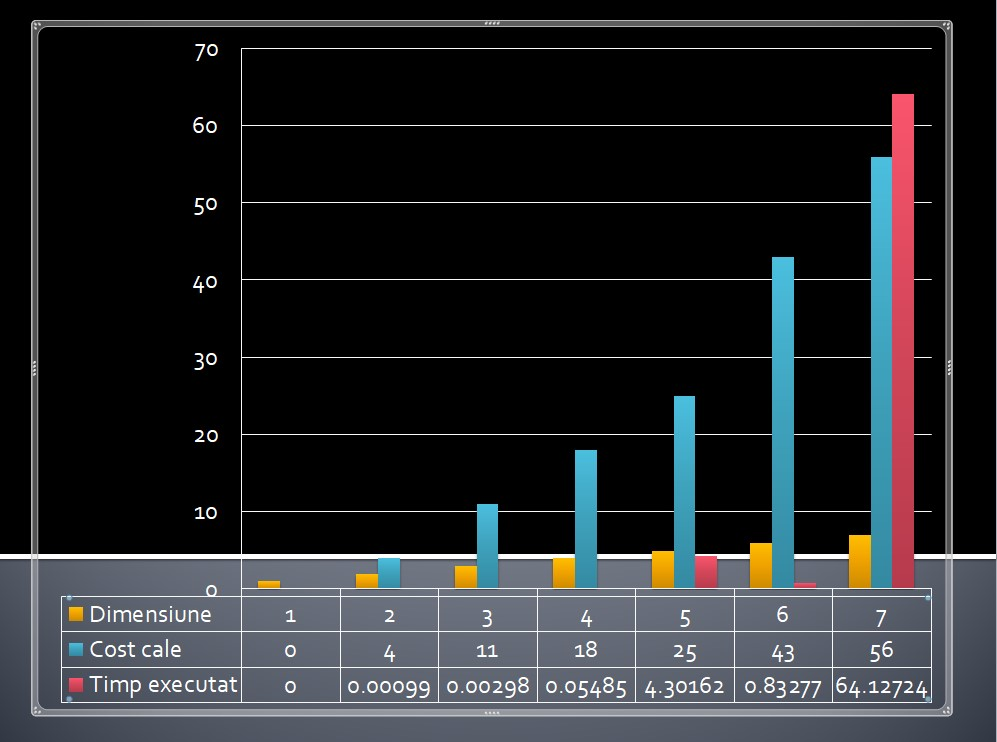
\includegraphics[width=12cm]{grafic-rezultate-obtinute.jpg}\\[0.8cm]
        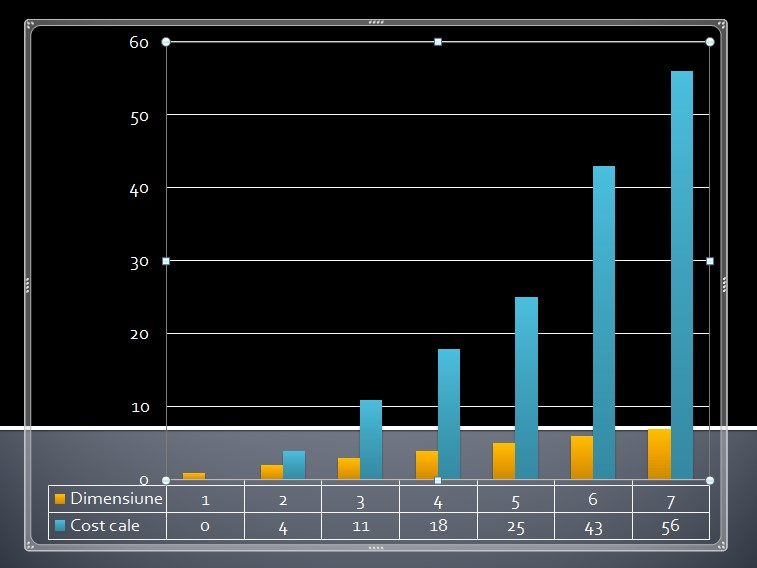
\includegraphics[width=12cm]{grafic-rezultate2.jpg}
        \bfseries \caption{\textbf{\textcolor{blue}{Grafice-Rezultate comparative pentru Astar-search}}}
\end{figure}
\begin{figure}
        \centering
        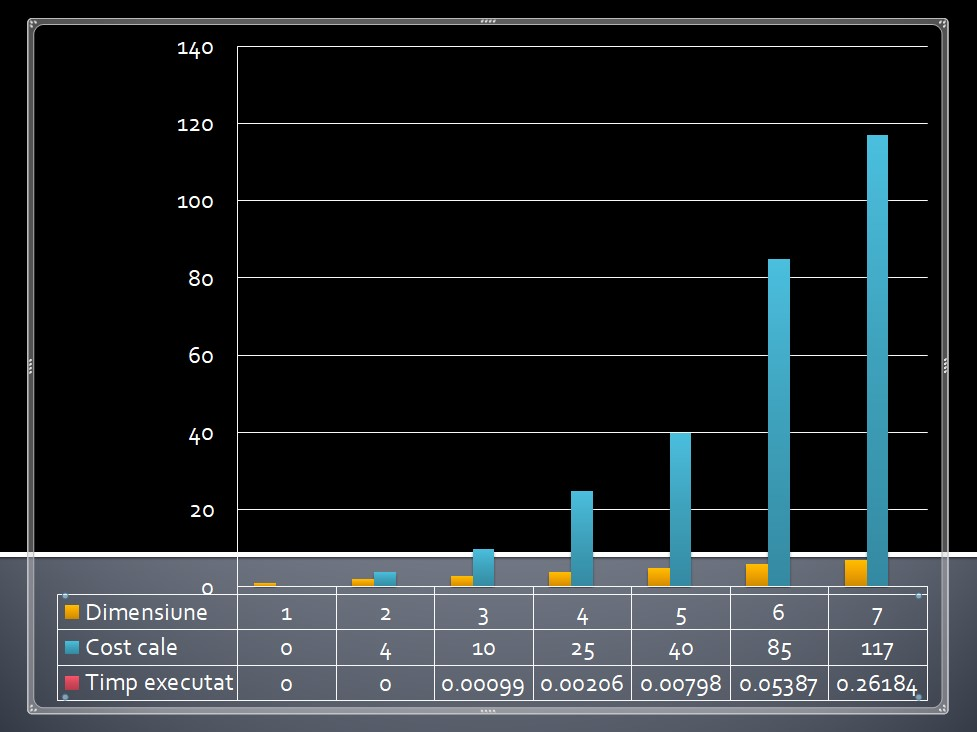
\includegraphics[width=12cm]{grafic-rezultate-bfs.jpg}\\[0.8cm]
        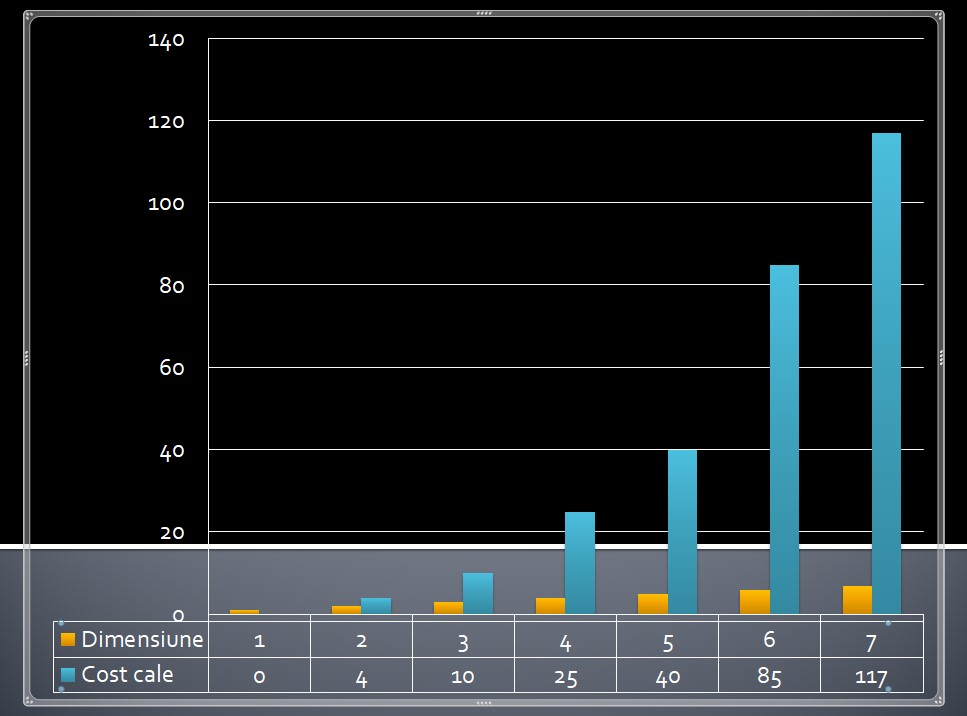
\includegraphics[width=12cm]{grafic_rezultate_bfs.jpg}
        \bfseries \caption{\textbf{\textcolor{blue}{Grafice-Rezultate comparative pentru Best-First-Search}}}
\end{figure}
\vspace{10mm}
\begin{center}
\begin{tabularx}{1\textwidth} { 
  | >{\raggedright\arraybackslash}X 
  | >{\centering\arraybackslash}X 
  | >{\centering\arraybackslash}X 
  | >{\raggedleft\arraybackslash}X  |}
\hline
\textcolor{blue}{\bfseries STAREA INITIALA } & \textcolor{blue}{\bfseries DIMENSIUNE PARCARE} & \textcolor{blue}{\bfseries NUMAR PASI EFECTUATI} & \textcolor{blue}{\bfseries STARE FINALA }\\
\hline
 \bfseries (0,2)  & \bfseries 2x2 & \bfseries 4  & \bfseries (3,1)  \\
\hline
 \bfseries (0,4,8,12) & \bfseries 4x4 & \bfseries 18 & \bfseries (15,11,7,3)\\
\hline
 \bfseries (0,6,12,18,24,30) & \bfseries 6x6 & \bfseries 43 & \bfseries (35,29,23,17,11,5)\\
\hline
 \bfseries (0,3,6) & \bfseries 3x3 & \bfseries 11 & \bfseries (8,5,2)\\
\hline
 \bfseries (0,5,10,15,20) & \bfseries 5x5 & \bfseries 25 & \bfseries (24,19,14,9,4)\\
\hline
 \bfseries (0,0) & \bfseries 1x1 & \bfseries 0 & \bfseries (0,0)\\
\hline
\bfseries (0,7,14,21,28,35,42) & \bfseries 7x7 & \bfseries 56 & \bfseries (48,41,34,27,20,13,6)\\
\hline 
\end{tabularx} 
\vspace{2mm}
   \quad \textbf{Date obtinute apeland functia pentru Astar search.} \par
\end{center} 
\vspace{5mm}
\begin{center}
\begin{tabularx}{1\textwidth} { 
  | >{\raggedright\arraybackslash}X 
  | >{\centering\arraybackslash}X 
  | >{\centering\arraybackslash}X 
  | >{\raggedleft\arraybackslash}X  |}
\hline
\textcolor{blue}{\bfseries STAREA INITIALA } & \textcolor{blue}{\bfseries DIMENSIUNE PARCARE} & \textcolor{blue}{\bfseries NUMAR PASI EFECTUATI} & \textcolor{blue}{\bfseries STARE FINALA }\\
\hline
 \bfseries (0,2)  & \bfseries 2x2 & \bfseries 4  & \bfseries (3,1)  \\
\hline
 \bfseries (0,4,8,12) & \bfseries 4x4 & \bfseries 25 & \bfseries (15,11,7,3)\\
\hline
 \bfseries (0,6,12,18,24,30) & \bfseries 6x6 & \bfseries 85 & \bfseries (35,29,23,17,11,5)\\
\hline
 \bfseries (0,3,6) & \bfseries 3x3 & \bfseries 10 & \bfseries (8,5,2)\\
\hline
 \bfseries (0,5,10,15,20) & \bfseries 5x5 & \bfseries 40 & \bfseries (24,19,14,9,4)\\
\hline
 \bfseries (0,0) & \bfseries 1x1 & \bfseries 0 & \bfseries (0,0)\\
\hline
\bfseries (0,7,14,21,28,35,42) & \bfseries 7x7 & \bfseries 117 & \bfseries (48,41,34,27,20,13,6)\\
\hline 
\end{tabularx}
\vspace{2mm}
   \quad \textbf{Date obtinute apeland functia pentru BEST-FIRST-SEARCH.} \par
   \vspace{10mm}
\end{center} 
\end{flushleft}
\textcolor{blue}{\subsection{\itshape\textcolor{blue}{Complexitatea computationala}}}
\quad\\ Pentru fiecare iteratie a buclei, A* trebuie sa determine calea pe care sa o extinda, astfel o face tinand cont de costul caii si a unei estimari a costului necesar pentru a extinde calea pana la obiectiv. Astfel costul total in orice etapa este suma costului pentru fiecare masina.\\ \par

\quad\\ Mutarea unei masini in orice directie implica un cost de 1, in timp ce statul pe loc al unei masini nu are cost. In cazul de fata pentru fiecare test, costul caii va fi altul, acesta reprezentand suma costului pentru fiecare masina, numarul de actiuni executate de fiecare vehicul. Cu cat dimensiunea parcarii, respectiv numarul de actiuni executate de fiecare vehicul creste, cu atat si costul caii creste.\\\par

\quad\\ A* calculeaza calea in functie de urmatoarea formula, adica selecteaza calea care minimizeaza:\\ \par
\vspace{25cm}

\textbf{\textcolor{red}{\bfseries{\\$ f(n)=g(n)+h(n) $}}}, unde:
\begin{itemize}
\bfseries
    \item \textcolor{red}{n} = nodul urmator de pe cale;
    \item \textcolor{red}{g(n)} = costul caii de la nodul initial pana la un nod final/obiectiv n;
    \item \textcolor{red}{h(n)} = functia euristica care estimeaza de fapt un cost mai ieftin pentru calea n pana la obiectiv, in cauzul nostru aceasta functie este chiar distanta Manhattan.
\end{itemize}
\vspace{2mm}
In tabelul prezentat mai jos, putem observa performanta, cat si complexitatea spatiului in cel mai rau caz.
\par
\begin{center}
\begin{tabular}{|p{4cm}|p{4cm}|}
    \hline
    \multicolumn{2}{|c|}{\bfseries A* search}\\
    \hline
    Performance&  Space complexity\\
    \hline
    \(O(|E|)=O(b^d)\)& \(O(|V|)=O(b^d) \)\\
    \hline
\end{tabular}
\end{center}
Factorul de ramificare poate fi determinat prin masurarea numarului de noduri N si adancimea solutiei, astfel: \textcolor{red}{$N+1=1+b^*+(b^*)^2+$\dots$+(b^*)^d$}, unde \textcolor{red}{$b^*$} = 1, iar \textcolor{red}{d} = numarul de actiuni executate in cazul problemei noastre, lungimea solutiei adica.\\
\vspace{10mm}
Best first search se implementeaza tratand multimea frontiera ca o coada cu prioritati avand drept functie de cost pe h(n). Va selecta la fiecare pas nodul din frontiera care “pare” a fi cel mai aproape de un nod obiectiv. Cu alte cuvinte se selecteaza nodul n care minimizeaza h(n). Best first search nu garanteaza intotdeauna gasirea unei solutii de cost minim.
\newline \\
In tabelul prezentat mai jos, putem observa performanta, cat si complexitatea spatiului in cel mai rau caz.
\begin{center}
\begin{tabular}{|p{4cm}|p{4cm}|}
    \hline
    \multicolumn{2}{|c|}{\bfseries Best first search}\\
    \hline
    Performance&  Space complexity\\
    \hline
    \(O(|E|)=O(b^m)\)& \(O(|V|)=O(b^m) \)\\
    \hline
\end{tabular}
\end{center}

\begin{center}
    \begin{figure}
        \centering
        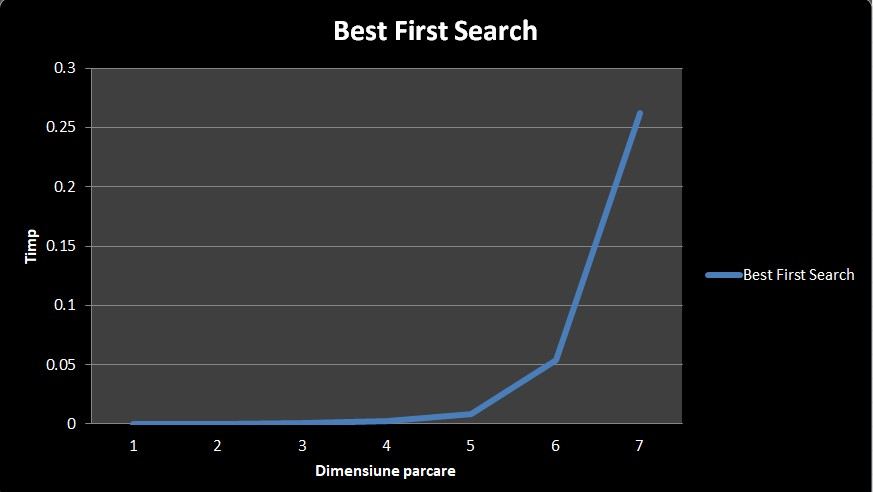
\includegraphics[width=15cm]{timp-best-first-search.jpg}
        \bfseries \caption{\textbf{\textcolor{blue}{Grafic-Timp executie Best first search}}}
    \end{figure}
\end{center}

\begin{center}
    \begin{figure}
        \centering
        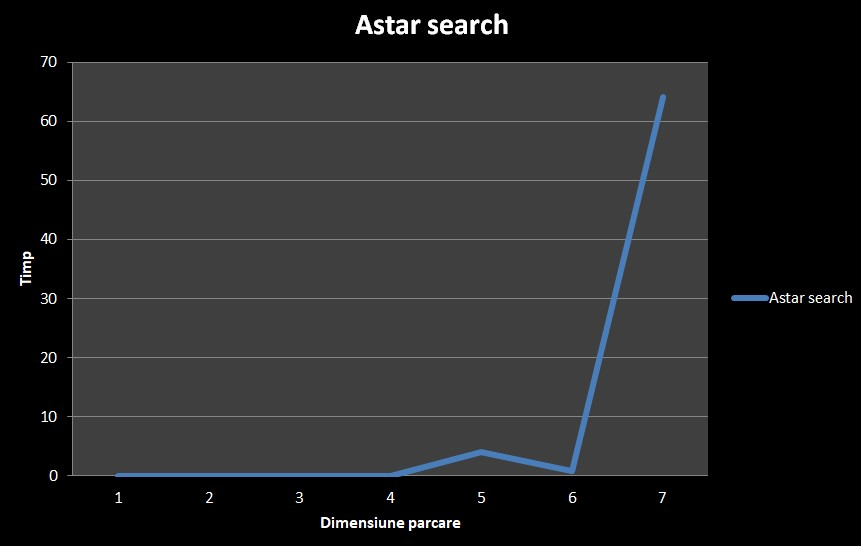
\includegraphics[width=15cm]{timp-astar-search.jpg}
        \bfseries \caption{\textbf{\textcolor{blue}{Grafic-Timp executie Astar search}}}
    \end{figure}
\end{center}

\begin{figure}
    \centering
    \begin{center}
      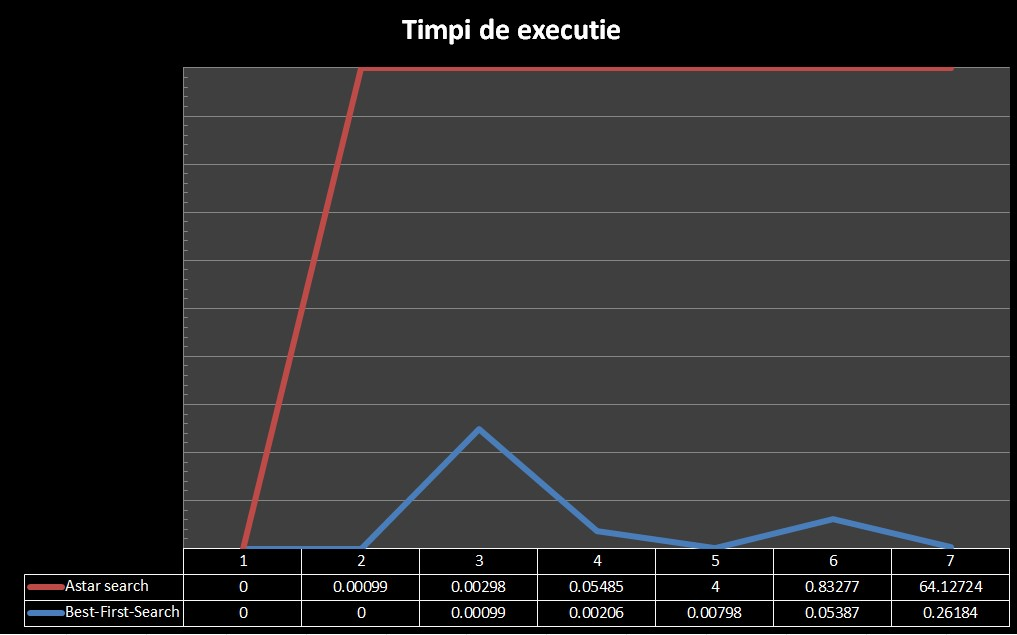
\includegraphics[width=15cm,height=10cm]{timpi-executie.jpg}
      \bfseries \caption{\textbf{\textcolor{blue}{Grafic comparativ intre timpii de executie}}}
    \end{center}
\end{figure}



Factorul de ramificare poate fi determinat prin masurarea numarului de noduri n si adancimea solutiei, astfel: \textcolor{red}{$T(n)=1+b+b^2+$\dots$+b^m$}, unde \textcolor{red}{$b$} = factor de ramificare, iar \textcolor{red}{d} = numarul de actiuni executate in cazul problemei noastre, lungimea solutiei adica.\\
\vspace{50cm}

\newpage
\textcolor{blue}{\subsection{\textcolor{blue}{Concluzii rezultate comparative}}}
\vspace{10mm}
\begin{itemize}
    \item Din cele doua tabele, respectiv din graficele atasate pe urmatoarele doua pagini se poate observa faptul ca utilizand best first search-ul avem un timp de executie mai mic, comparativ cu timpul de executie obtinut cand folosim astar search;
    \newline 
    \item Se poate observa ca atunci cand apelam functia astar search, costul caii este mult mai mic, inclusiv numarul de pasi efectuati de fiecare vehicul pentru a ajunge la starea finala, dar timpul de executie este mult mai mare;
    \newline
    \item Ambii algoritmi genereaza acelasi rezultat, dar difera costul caii, actiunile executate de fiecare vehicul, cat si timpul executat pentru a ajunge la starea finala;
    \item Ambii algoritmi apeleaza functia pentru distanta Manhattan care calculeaza euristica pentru problema cautarii in programul nostru;
    \newline
    \item Un avantaj al utilizarii Best First Search in problema noastra este dat de viteza mai mare de a ajunge la starea finala;
    \newline
    \item Un dezavantaj al utlizisarii Astar search in problema noastra este utilizarea unei cantitati mari de timp;
    \newline
    \item Din primul grafic realizat, se poate observa ca atunci cand dimensiunea parcarii este \\ \emph 1 x \emph 1, timpul executat, cat si costul caii sunt 0, cu cat dimensiunea parcarii este mai mare rezulta ca si timpul executat creste, respectiv si costul caii. Se poate observa o crestere semnificativa a timpului de executie pentru o dimensiune de \emph 7 x \emph 7 a parcarii, \emph 7 x \emph 7 fiind si ultima valoare obtinuta pentru care algoritmul ofera un raspuns. Rezultatele din primul grafic sunt pentru algoritmul de cautare Astar search;
    \newline
    \item Din al doilea grafic realizat, se poate observa ca atunci cand dimensiunea parcarii este \\ \emph 1 x \emph 1, timpul executat, cat si costul caii sunt 0, cu cat dimensiunea parcarii este mai mare rezulta ca si timpul executat creste cate putin, respectiv si costul caii. Se poate observa o crestere semnificativa a costului pentru cale la o dimensiune de \emph 7 x \emph 7 a parcarii, \emph 7 x \emph 7 fiind si ultima valoare obtinuta pentru care algoritmul ofera un raspuns. Rezultatele din al doilea grafic sunt pentru algoritmul de cautare BEST-FIRST-SEARCH.
    \newline
\end{itemize}
\end{flushleft}
\newpage
\vspace{5mm}
\quad Daca ar fi sa presupunem ca avem o parcare de \emph 4 x \emph 4 si \emph 4 vehicule in aceasta parcare, numerotate cu cifrele 1, 2, 3, 4 pentru a ajunge la obiectivul nostru, aceste vehicule ar trebui sa execute mai multe mutari astfel incat la final sa fie asezate in ordine inversa.\\

\begin{figure}
    \centering
    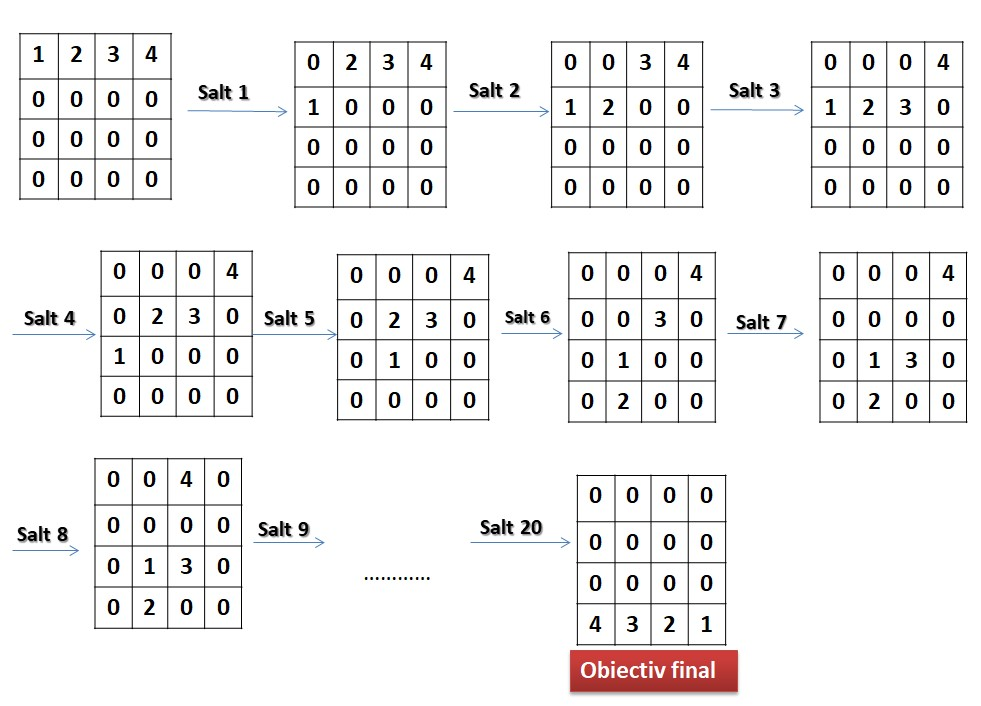
\includegraphics[width=15cm]{salturi-posibile.jpg}
    \bfseries\caption{\textbf{\textcolor{blue}{Succesiunea de miscari de la starea initiala la starea finala}}}
    \vspace{1cm}
\end{figure}
Mai sus este prezentata o diagrama realizata in PowerPoint cu scopul de a evidentia  numarul de salturi efectuate de cele \emph 4 vehicule pana la obiectivul final.
Se poate observa ca pentru o dimensiune de \emph 4 x \emph 4, cele \emph 4 vehicule executa 20 de salturi/mutari pana ajung la obiectivul final, deoarece fiecare vehicul poate executa cel mult 5 miscari/salturi posibile din orice pozitie.\\\\ Starea din care pornesc nu se adauga la numaratoare, deoarece reprezinta starea initiala, starea din care vehiculele incep sa execute salturile, astfel fiind dat starea initiala reprezinta de fapt pozitia fiecarui vehicul, iar starea finala reprezinta pozitiile in care trebuie sa ajunga fiecare dintre vehiculele noastre la randul de sus, dar in ordine inversa. Astfel aceste salturi, respectiv mutari pot fi privite ca actiuni, acestea reprezentand actiunile pe care fiecare vehicul le poate executa in functie de locatia sa in parcare si de pozitia altor vehicule.\par
\newpage
\begin{flushleft}
\begin{center}
    \textcolor{blue}{\section{\bfseries\scshape\textcolor{blue}{Concluzii finale}}}
    \vspace{5mm}
\end{center}
\end{flushleft}
\begin{flushleft}
    \begin{itemize}
        \item Consider ca aceasta tema a reprezentat o provocare(din care am incercat sa invat si sa acumulez cat mai multe detalii, notiuni), atat intelegerea cerintei, abordarea problemei, cat si implemenatarea algoritmului.
        \vspace{2mm}
        \item In urma acestei teme, mi-am imbunatatit abilitatile de coding in limbajul Python, cat si notiunile de sintaxa in LaTex.
        \vspace{2mm}
        \item O alta experienta a reprezentat-o adaptarea problemei din tema de casa folosind framework-ul de la 15-puzzle problem aferent laboratorului 5. Aceasta a reprezentant cea mai mare provocare, atat modificarea si adaptarea codului, cat si gasirea unei functii euristice admisibile in raport cu cerinta temei de casa, deoarece fiecare vehicul executa maxim 5 actiuni.
        \vspace{2mm}
        \item Am ales sa dezvolt implementarea in limbajul Python, deoarece modalitatea de implementare in acest limbaj este mai usor de inteles, si mi-am dorit sa imi imbunatatesc mai mult abilitatile in acest limbaj.
        \vspace{2mm}
       \item Consider ca euristica pe care am folosit-o in cadrul acestei rezolvari ofera cel mai admisibil rezultat pentru aceasta problema. Dar cred ca in viitor acest algoritm se poate imbunatati mai mult, astfel incat sa functioneze cat mai optim.
       \vspace{2mm}
       \item Ca o extindere a studiului pe termen mai lung, consider ca referinta ajutatoare in intelegerea si parcurgerea temelor de casa, cartea Artificial Intelligence: A Modern Approach, Fourth edition, 2020 by Stuart Russell and Peter Norvig, cat si materialele auxiliare din platformele de laborator, sau din cadrul cursurilor aferente acestei discipline.
       \vspace{2mm}
       \item In scopul rezolvarii acestei probleme, cel mai mult m-a ajutat framework-ul de la 15-puzzle problem, cat si materialele auxiliare din platforma de laborator 5 pentru a intelege mai bine cerinta problemei, cat si pentru o abordare mai ampla a rezolvarii.
       \vspace{2mm}
       \item O alta concluzie este reprezentata de termenul limita al temei de casa. Acest parametru a avut un impact mai bun asupra organizarii timpului, cat si asupra unei coordonari mai responsabile a celorlalte aspecte realizate pentru a rezolva aceasta tema, ceea ce constituie un beneficiu mai amplu pentru dezvoltarea mea in acest domeniu.
       \vspace{2mm}
       \item  Am incercat sa respect fiecare cerinta din metodologie, astfel incat sa pot descrie fiecare parametru corespunzator acesteia in functie de implementarile, abordarea si rezultatele pe care le-am justificat mai sus.
    \end{itemize}
\end{flushleft}

\newpage
\begin{flushleft}
\begin{center}
      \textcolor{blue}{\section{\bfseries\scshape\textcolor{blue}{Bibliografie}}}
      \vspace{2mm}
\end{center}
\end{flushleft}
\begin{flushleft}
    \quad Mai jos se pot observa cateva referinte bibliografice, capitole din cursuri, carti, site-uri web, referinte ce au ajutat in parcurgerea, documentarea si intelegerea mai ampla a temei de casa. De pe site-urile respective m-am documentat, link-urile sunt atasate mai jos: \par
\begin{thebibliography}{8}
\bfseries\scshape
        \bibitem{aima-website} 
         Artificial Intelligence: A Modern Approach, Fourth edition, 2020 by Stuart Russell and Peter Norvig,
        \textcolor{blue}{\\\url{http://aima.cs.berkeley.edu/}}
        \bibitem{overleafwebsite} 
        Introducing Overleaf and LaTeX,
        \textcolor{blue}{\\\url{https://www.overleaf.com/learn/latex/Tutorials}
        \\\url{https://oeis.org/wiki/List_of_LaTeX_mathematical_symbols}
        \\\url{https://mirrors.nxthost.com/ctan/macros/latex/required/graphics/grfguide.pdf}
        \\\url{https://sharelatex.psi.ch/learn/XeLaTeX}}
        \bibitem{python-website} 
        Python Documentation contents,
        \textcolor{blue}{\\\url{https://www.w3schools.com/python/}
        \\\url{http://www.pacosv.ro/informatica/Fisiere_Python.pdf}
        \\\url{http://docs.groovy-lang.org/next/html/documentation/working-with-collections.html}
        \\\url{https://stackoverflow.com/questions/37400974/unicode-error-unicodeescape-codec-cant-decode-bytes-in-position-2-3-trunca}}
        \bibitem{capitol-curs} 
         Capitolul 5 din curs\\
         Capitolul 6 din curs - Cautare euristica
        \bibitem{laborator}
         Laborator 5 - Cautare informata folosind Python
        \bibitem{problem-introduction} 
        Heuristicars Problem 
        \textcolor{blue}{\\\url{http://www.cs.cmu.edu/afs/cs/academic/class/15780-s15/www/hw/hw1key.pdf}
        \\\url{https://ai.stackexchange.com/questions/18355/if-h-i-are-consistent-and-admissible-are-their-sum-maximum-minimum-and-aver}}
        \bibitem{aima} 
        Solving problems by searching,
        \textcolor{blue}{\\\url{https://www.pearsonhighered.com/assets/samplechapter/0/1/3/6/0136042597.pdf}
        \\\url{https://people.cs.pitt.edu/~milos/courses/cs1571/Lectures/Class3.pdf}
        \\\url{https://xlinux.nist.gov/dads/}
        \\\url{https://www.geeksforgeeks.org/a-search-algorithm/}}
        \bibitem{github}
        Pseudocode descriptions of the algorithms,
        \textcolor{blue}{\\\url{https://github.com/aimacode/aima-pseudocode/blob/master/aima3e-algorithms.pdf}
        \\\url{https://github.com/ishaansharma/AIMA-Solutions}}
        \bibitem{AI}
        Inteligenta Artificiala-Rezolvarea problemelor de cautare,
        \textcolor{blue}{\\\url{http://www.cs.ubbcluj.ro/~lauras/test/docs/school/IA/2018-2019/lectures/01_search_uninformed.pdf}}
        \bibitem{Grid}
        Visualization a grid,
        \textcolor{blue}{\\\url{https://cse442-17f.github.io/A-Star-Search/}
        \\\url{https://www.redblobgames.com/grids/hexagons/distances}}
        \vspace{15cm}
\end{thebibliography}
\large \textcolor{blue}{\bfseries{$\copyright$}} Iunie 2021.
\end{flushleft}





\end{document}